\documentclass[11pt]{article}
\usepackage[utf8]{inputenc}

\usepackage{authblk}

\title{Vehicle Routing Problems in the Age of Semi-Autonomous Driving}
\author[1]{Hins Hu}
\author[2]{Samitha Samaranayake}
\affil[1]{{\small Systems Engineering, Cornell University, zh223@cornell.edu}}
\affil[2]{{\small School of Civil and Environmental Engineering, Cornell University, samitha@cornell.edu}}
\date{}

% --- Colors ---
\usepackage[dvipsnames]{xcolor}
\definecolor{cornellred}{HTML}{B31B1B}

% --- Drawing ---
\usepackage{tikz}
\usepackage{tikz-network}
\usetikzlibrary{backgrounds}
\usetikzlibrary{patterns}

\usepackage{pgfplots}
\pgfplotsset{width=10cm,compat=1.9}
% \usepgfplotslibrary{external}
% \tikzexternalize

% --- Math ---
\usepackage{amsmath}
\usepackage{amssymb}
\usepackage{amsthm}
\usepackage{bm}
\usepackage{mathtools}
\DeclareMathOperator*{\argmax}{arg\,max}
\DeclareMathOperator*{\argmin}{arg\,min}
\usepackage{thmtools, thm-restate}
\usepackage{optidef}

% --- Figures ---
\usepackage{graphicx}

% --- Fonts ---
\usepackage{amsfonts}

% --- Algorithm ---
\usepackage{algorithm}
\usepackage{algpseudocode}
\renewcommand{\algorithmicrequire}{\textbf{Input:}}
\renewcommand{\algorithmicensure}{\textbf{Output:}}


% --- Comments ---
\newcommand{\Hins}[1]{{\color{blue}([Hins] #1)}}
\newcommand{\SSC}[1]{{\color{red}([Samitha:] #1)}}


% --- Bibliography
\usepackage[style = numeric]{biblatex}
\addbibresource{references.bib}
% \bibliographystyle{unsrt}  % or another preferred BibTeX style
% \bibliography{references}


% --- blocks
\newtheorem{remark}{Remark}[section]
\newtheorem{example}{Example}[section]

\newtheorem{theorem}{Theorem}[section]
\newtheorem{corollary}[theorem]{Corollary}
\newtheorem{lemma}[theorem]{Lemma}
\newtheorem{proposition}[theorem]{Proposition}
\newtheorem{definition}{Definition}[section]
% \setcounter{section}{0}

% --- Layout ---
\usepackage{caption}
\usepackage{subcaption}
\usepackage{longtable}
\usepackage[top = 1in, bottom = 1in, left = 1in, right = 1in]{geometry}
\setlength{\parskip}{0.1em}
\usepackage{multirow}
\usepackage{setspace}
\onehalfspacing

% --- hyper link ---
% \usepackage[pdftex, hidelinks]{hyperref}
\usepackage[colorlinks=true,linkcolor=black,citecolor=black,urlcolor=black,
            pdfauthor={},pdftitle={},pdfproducer={},pdfcreator={}]{hyperref}


\begin{document}



\maketitle

\begin{abstract}
We are in the midst of a semi-autonomous era in urban transportation in which varying forms of vehicle autonomy are gradually being introduced. This phase of partial autonomy is anticipated by some to span a few decades due to various challenges, including budgetary constraints to upgrade the infrastructure and technological obstacles in the deployment of fully autonomous vehicles (AV) at scale. In this study, we introduce the \textit{vehicle routing problem in a semi-autonomous environment} (VRP-SA) where the road network is not fully AV-enabled in the sense that a portion of it is either not suitable for AVs or requires additional resources in real-time (e.g., remote control) for AVs to pass through. Moreover, such resources are scarce and usually subject to a budget constraint. An exact mixed-integer linear program (MILP) is formulated to minimize the total routing cost of service in this environment. We propose a two-phase algorithm based on a family of \textit{feasibility recovering sub-problems} (FRP) to solve the VRP-SA efficiently. Our algorithm is implemented and tested on a new set of instances that are tailored for the VRP-SA by adding stratified grid road networks to the benchmark instances. The result demonstrates a reduction of up to 37.5\% in vehicle routing costs if the fleet actively exploits the AV-enabled roads in the environment. Additional analysis reveals that cost reduction is higher with more budget and longer operational hours.
\end{abstract}


\section{Introduction}
With the development of numerous advanced technologies related to autonomous driving, such as smart sensors, computer vision, and high-speed wireless communication, the deployment of autonomous vehicles (AV) fleets in all kinds of transportation is becoming more and more viable. More importantly, replacing human-driven vehicles (HDV) with AVs in many businesses may potentially reduce the operational cost dramatically as drivers' wages contribute a great portion of it. In the trucking industry, according to a report \cite{leslie2022analysis}  by the American Transportation Research Institute, the driver-based cost contributed 35.8\% of the average marginal cost per mile in 2011 and this number climbed up to 40.2\% in 2022 due to increases in labor costs. If we deduct the amortized cost of vehicle purchases and leases, the percentage of the driver-based cost to the operational cost per mile in 2011 and 2019 are 37.6\% and 47.2\% respectively.

Although the AV industry has seen significant advancements and substantial investment, a fully autonomous driving environment remains years away. The era of \textit{semi-autonomous driving} is expected to persist for several decades due to numerous barriers. First, key technologies such as motion planning and object detection continue to pose significant bottlenecks. According to SAE International’s classification system \cite{sae2018taxonomy}, autonomous driving is categorized into six levels, ranging from level 0 (no automation) to level 5 (full automation). As of March 2021, Honda became the first manufacturer to offer a legally approved level-3 vehicle \cite{Honda2021}, capable of autonomous driving in certain conditions, though human intervention is still required in some situations. Second, mixed traffic environments, with both AVs and HDVs, are inevitable due to factors such as consumer preference and the long service life of traditional automobiles. A survey on commuting preferences \cite{HABOUCHA201737} conducted with 721 participants found that many individuals remain hesitant to adopt AVs. Even with a fully subsidized shared AV service, 44\% of respondents still preferred regular vehicles, and only 75\% expressed interest in switching to shared AVs. Third, achieving full automation in some scenarios is more challenging than in others. For example, high-density urban areas, compared to long-haul truck platooning, present greater complexity for level-5 automation due to intricate road networks, frequent interactions between vehicles and pedestrians, and the existence of traffic control. Fourth, autonomous driving requires significant infrastructure upgrades, particularly in vehicle-to-infrastructure (V2I) communication systems, to facilitate precise AV maneuvers such as lane-changing and merging. However, the investment required for these upgrades is often constrained by budgetary limitations, making it a long-term undertaking. Finally, legislative and policy frameworks tend to lag behind technological development. Concerns around safety, equity, and privacy often drive a more conservative approach to regulating autonomous driving, further delaying widespread adoption.

Given the limitations aforementioned, new challenges arise when deploying AVs in a semi-autonomous environment. Specifically, road networks are not fully accessible to AV fleets in the sense that certain levels of AVs may be prohibited from traversing a subset of road segments, leading to a classification of roads based on their compatibility with different levels of AV autonomy. In the simplest case, the road network can be modeled as a bi-level system comprising \textit{ordinary roads} and \textit{AV-enabled roads}. Additionally, a critical feature of the semi-autonomous environment is that not all AVs operate at full autonomy (i.e., level 5). Some may require external resources, such as real-time remote control, to navigate AV-enabled roads. These resources, however, are typically costly. For instance, in October 2020, Waymo launched a geo-fenced semi-autonomous ride-hailing service in Phoenix, U.S., supported by a team of remote engineers available to intervene in contingencies \cite{Waymophoenix}. Similarly, Enride has deployed electric autonomous trucks on low-traffic private roads within logistics and manufacturing hubs and is working toward operating them on public roads with remote supervision \cite{enride2022}.

With that said, optimal vehicle dispatching and routing strategies at the operational level, traditionally modeled by the vehicle routing problem (VRP), need to be re-examination and re-designed, particularly for high-density urban areas. Moreover, vehicle dispatching schedules are crucial because the simultaneous demand for resources by all AVs must not exceed the maximum capacity. Exceeding this capacity can result in system failures with severe consequences, such as collisions. From a resource allocation perspective, fleet operators need to assign resources to AVs effectively by designing vehicle schedules based on prior knowledge of road networks. To address these new challenges, a holistic optimization approach is essential. Therefore, we propose a novel variant of the VRP, termed the \textit{Vehicle Routing Problem in the Semi-Autonomous Environment} (VRP-SA).

\textbf{The contribution of our work is threefold:} (1) We formalize a novel vehicle routing problem called VRP-SA to address the new challenges of deploying AV fleets in a semi-autonomous environment. (2) We provide a practically efficient solution approach for the VRP-SA. (3) We analyze the impact of varying unit routing costs and the density of AV-enabled roads on the deployment of AVs in the age of semi-autonomous driving.

The paper is organized as follows: Section \ref{sec:literature} briefly reviews the history of VRP and relevant literature on VRP variants involving mixed fleets and limited resources. Section \ref{sec:description} presents a formal description of the VRP-SA. Section \ref{sec:milp} introduces an exact mixed-integer linear program (MILP) for the VRP-SA. Section \ref{sec:milp_extend} discusses some extended studies in the MILP to enhance the model's comprehensiveness and adaptability. Section \ref{sec:algo} presents a two-phase algorithm based on a family of feasibility recovering sub-problems (FRP) to solve the VRP-SA efficiently. Section \ref{sec:exp} presents a new set of instances tailored for the VRP-SA and analyzes the results of numerical experiments conducted on these instances. Section \ref{sec:conclusion} concludes the paper and outlines potential directions for future research.



\section{Literature Review} \label{sec:literature}
VRP was first formulated as an integer linear program by Dantzig and Ramser \cite{dantzig1959truck} in 1959. The seminal heuristic algorithm to solve it was developed by Clark and Wright \cite{clarke1964scheduling} in 1964. The proof of the NP-hardness of VRP was provided by Lenstra and Kan \cite{lenstra1981complexity} in 1981. In addition to these milestones, extensive studies in VRP models (e.g. \cite{golden1984fleet}
\cite{kolen1987vehicle} \cite{savelsbergh1995general}
\cite{renaud1996tabu} \cite{erdougan2012green}
\cite{schneider2014electric}), construction heuristics (e.g. \cite{gillett1974heuristic} \cite{fisher1981generalized} \cite{bramel1995location}), meta-heuristics (e.g. \cite{homberger1999two} \cite{bell2004ant} \cite{pisinger2007general}), branch-and-bounds approaches (i.e., \cite{desrochers1992new} \cite{fischetti1994branch} \cite{fukasawa2006robust}), and learning-based approaches (e.g. \cite{nazari2018reinforcement} \cite{kool2018attention} \cite{li2021learning}) have been conducted and published over the past decades. Numerous benchmark data sets (e.g. \cite{solomon1987algorithms} \cite{augerat1995computational} \cite{uchoa2017new}) have also been created to support the performance tests of newly-developed VRP algorithms. The most recent research on VRP follows a trend toward designing a general-purpose algorithm by the hybridization of various frameworks to solve a wide range of VRP variants efficiently and on a larger scale. The representative work is the unified hybrid genetic search (UHGS) developed by Vidal et al. \cite{VIDAL2014658}. More comprehensive literature reviews from different aspects of VRP are referred to these papers (\cite{braysy2005vehicle_1} \cite{braysy2005vehicle_2} \cite{montoya2015literature} \cite{kocc2016thirty} \cite{lin2014survey} \cite{braekers2016vehicle}) and this book \cite{toth2014vehicle}.

A key feature of the VRP-SA is its mixed fleet of AVs and HDVs, which can be modeled by the family of Heterogeneous Fleet Vehicle Routing Problems (HFVRP) involving only two types of vehicles. This topic is covered in a chapter by Toth and Vigo \cite{toth2014vehicle}. The HFVRP family can be further refined into different categories depending on fleet constraints (limited or unlimited) and cost structures (vehicle-dependent or vehicle-independent). Research on exact approaches for the HFVRP is relatively limited. The most effective exact approach currently available is the branch-and-cut-and-price algorithm developed by Baldacci and Mingozzi \cite{baldacci2009unified}. In contrast, most existing approaches are heuristic-based, such as the multi-start adaptive memory programming (MAMP) by Li et al. \cite{LI20101111}, the variable neighborhood search (VNS) by Imran et al. \cite{IMRAN2009509}, and the memetic algorithms by Prins \cite{PRINS2009916}. Currently, the UHGS approach \cite{VIDAL2014658} is recognized as the leading method for the HFVRP.

One recent work by Molina et al. \cite{MOLINA2020103745} also discussed the VRP with a limited number of resources available. However, their focus is on scenarios where resource limitations—such as drivers, vehicles, or other equipment—prevent the servicing of all customers. This contrasts with our work, where limited resources (e.g., remote control) shared across the entire AV fleet can influence the routing decisions of individual vehicles when serving multiple customers.


\section{The Problem Statement of VRP-SA} \label{sec:description}
The VRP-SA admits the following inputs: (1) A directed graph $G = (V, E = E^a \cup E^o)$ representing the underlying road network, where $V$ is the set of nodes representing road intersections, and $E^a$ and $E^o$ are the sets of edges representing AV-enabled and ordinary road segments, respectively. (2) A depot $o \in V$ from which all vehicles depart and to which they return after the service. (3) A time horizon $[0, T]$ of operations (e.g., a day). (4) A set of customers $D \subset V$ with a demand vector $\bm{d} \in \mathbb{R}^{|D|}_{++}$. (5) A mixed vehicle fleet $M = M^a \cup M^h$, where $M^a$ is the set of AVs and $M^h$ is the set of HDVs, all with identical capacity $W \in \mathbb{R}_{++}$. (6) A pair of fixed costs $(f^a, f^h)$ of dispatching an AV and an HDV, respectively. (7) A vector of routing costs $\bm{c} \in \mathbb{R}_{++}^{3 \times |E|}$, where each cost is associated with a road segment in $E$ and varies by vehicle type and road type. The cost structure is detailed in Table \ref{tab:cost}. Here, $c_e^1$ and $c_e^2$ represent the routing costs for an AV traveling on an AV-enabled road segment $e \in E^a$ and an ordinary road segment $e \in E^o$, respectively. Similarly, $e_e^0$ denotes the routing cost for an HDV traversing any road $e \in E$, regardless of type. Two constant cost adjustment factors, $\eta_1$ and $\eta_2$, are applied uniformly across all edges. (8) A vector of travel times $\Delta \bm{t} \in \mathbb{R}_{++}^{|E|}$, with each entry corresponding to a road segment. (9) A budget $B \in \mathbb{N}_+$ representing the number of remote controllers available to assist AVs in real-time while they are traversing ordinary road segments. All aforementioned notations are summarized in Table \ref{tab:notations} for reference in later sections.
\begin{table}[!htbp]
    \centering
    \begin{tabular}{|c|c|c|}
        \cline{1-3}
         & AV-Enabled Roads & Ordinary Roads\\ \hline
        AVs & $c^{1}_e = \eta_1 \cdot c^0_e$ & $c^{2}_e = \eta_2 \cdot c^0_e$ \\ \hline
        HDVs & $ c^0_e$ & $ c^0_e$ \\ \hline
    \end{tabular}
    \caption{The routing cost structure of a vehicle traversing road segment $e$}
    \label{tab:cost}
\end{table}

The problem is subject to the following assumptions: (1) HDVs can traverse the entire road network freely without external resources, whereas AVs require additional support from remote controllers to pass through ordinary roads. Specifically, an AV locks one remote controller upon entering an ordinary road from an AV-enabled road and releases it upon returning to an AV-enabled road. (2) As outlined in Table \ref{tab:cost}, the routing cost for a vehicle on a given road segment depends on both the vehicle and road types. We further assume that, in the age of semi-autonomous driving, the routing cost for an AV on an AV-enabled road is lower than that for an HDV on the same road (i.e., $\eta_1 < 1$). Conversely, on an ordinary road, the cost for an AV exceeds that of an HDV (i.e., $\eta_2 > 1$). This assumption is justified by the significant cost reduction from eliminating driver-related expenses on AV-enabled roads. However, on ordinary roads, the scarcity and high cost of remote controllers lead to increased operational expenses, surpassing even the driver-related portion. (3) The dispatched times for vehicles are flexible within $[0, T]$, provided that all vehicles return to the depot before $T$.

The objective of the VRP-SA is to find a minimum-cost dispatching and routing strategy that serves all customers while satisfying the budget constraint of remote controllers, the return time constraints, and the capacity constraints. The fixed costs for establishing the real-time remote control system are treated as overheads and thus excluded from our decision making. Additionally, we do not integrate other commonly seen conventional constraints, such as time windows for customers and the order of pick-up and delivery, as they are relatively independent of the core issues addressed in this paper.

\section{The Mixed-Integer Linear Program} \label{sec:milp}
In this section, we will first briefly discuss a challenge of formulating the VRP-SA as a mixed-integer linear program (MILP). Next, we will establish a connection between a key characteristic of the VRP-SA and a simpler classical combinatorial optimization problem known as the \textit{Steiner Traveling Salesman Problem} (STSP). Leveraging several properties of the STSP, we will then demonstrate how to construct an \textit{expanded graph} based on the original road network and derive an exact MILP formulation for our problem on this expanded graph.

Many VRP models and algorithms are formulated and designed based on the \textit{metric closure} of the underlying road network \cite{toth2014vehicle}. The metric closure of a graph $G$ on a subset of nodes $D$ is a complete graph $\overline{G}$ on $D$, where each edge is weighted by the cost of the shortest path between the two corresponding nodes in $G$. This transformation allows each vehicle route in the solution to be represented as an ordered sequence, indicating the order of serving the subset of customers assigned to that vehicle. The low-level routing in the real-world road network is pre-determined by computing the minimum-cost paths between all pairs of customers. This trick significantly reduces the number of decision variables and constraints required to model a VRP, resulting in a more compact formulation. For instance, it ensures that each customer node is visited exactly once in the optimal solution, enabling the use of a constraint akin to unit flow conservation \cite{dantzig1959truck}. This pre-processing step, which transforms the underlying network into its metric closure, is illustrated in Figure \ref{fig:metric_closure}.

However, this trick is not applicable to the VRP-SA due to the presence of mixed road types in the underlying network. While shortest paths can still be pre-determined, a vehicle may not always travel along the shortest path between two customers in the optimal solution. This is because its ability to navigate an ordinary road segment depends on the continuous availability of a remote controller during the entire period it remains on the segment, from entry to exit. Consequently, the feasibility of selecting ordinary road segments for different AV routes is interdependent and constrained by a real-time enforced budget. Figure \ref{fig:metric_closure} further demonstrates that, once the network is transformed into its metric closure, all information about the road type of each edge is lost.
\begin{figure}[htbp!]
    \centering
    \includegraphics[width=0.9\linewidth]{metric_closure_2.png}
    \caption{A toy example of a road network of mixed road types and its metric closure}
    \label{fig:metric_closure}
\end{figure}

Therefore, to formulate an MILP for the VRP-SA, we must work directly on the original road network. A key characteristic of an optimal solution to the VRP-SA in the original network is that any node may be visited more than once if necessary, which features the STSP in its most basic form. The formal definition of the STSP is as follows: Given an undirected and connected graph, a subset of nodes designated as required nodes to be served, a distinguished required node serving as the depot, and positive costs associated with all edges, the objective is to determine a minimum-cost route that visits all required nodes. Essentially, the Steiner version of the TSP relaxes the requirement for the graph to be complete \cite{RODRIGUEZPEREIRA2019615}. We identify the following two lemmas of the STSP, with formal proofs provided in Appendix \ref{app: A}.

\begin{restatable}{lemma}{lemmanode} \label{lemma:1}
In an optimal solution to the STSP in a directed graph, a node can be visited at most $n$ times, where $n$ is the number of required nodes in the graph. 
\end{restatable}

\begin{restatable}{lemma}{lemmaedge} \label{lemma:2}
In an optimal solution to the STSP in a directed graph, an edge can be traversed at most $n-1$ times, where $n$ is the number of required nodes in the graph.
\end{restatable}

The observations in Lemma \ref{lemma:1} and Lemma \ref{lemma:2} can be naturally extended to the VRP-SA. Specifically, for each node in the set \( V \), an upper bound on the number of times it can appear in an optimal solution to the VRP-SA can be established. This result is presented in Proposition \ref{prop: k}, with a detailed proof provided in Appendix \ref{app: A}.

\begin{restatable}{proposition}{propositionk} \label{prop: k}
Let $P(m)$ be the route of vehicle $m$ in the optimal solution to the VRP-SA. Let $W$ be the capacity of vehicle $m$. Let $\{d_i: \; i = 1, \dots, |D| \}$ be a non-decreasing sequence indicating the demands of customer set $D$. Then, a node $v \in P(m)$ can be visited by vehicle $m$ at most $k + 1$ times, and an edge $(u, v), \; \forall \; u, v \in P(m)$ can be traversed by vehicle $m$ at most $k$ times, where $k$ is defined as the largest integer $j = 1, \dots, |D|$ satisfying $\sum_{i=1}^j d_i \leq W$.
\end{restatable}

Building on the result of Proposition \ref{prop: k}, we propose an approach to formulate an exact MILP for the VRP-SA by constructing a \textit{$k$-layer expanded graph} $G_e$ from the original network graph $G$, where $k$ is the number defined in Proposition \ref{prop: k}. The construction process is as follows:
\begin{enumerate}
    \item Duplicate $G$ by $k$ times and stack them in layers.
    \item Create an dummy node $s$ called the \textit{sink depot} on the base layer. 
    \item For every two adjacent layers, add an dummy directed edge pointing from every customer on the lower layer to its duplicate customer on the upper layer.
    \item For every duplicate depot on the duplicate layers, add an dummy directed edge pointing from the depot to the sink depot $s$.
    \item Assign zero cost and zero travel time to each dummy edge. 
\end{enumerate}

Accordingly, additional notations are introduced to account for duplication in the expanded graph and to support the MILP formulation later in this section. These notations are clearly explained and summarized in Table \ref{tab:notations}, so their definitions will only be repeated in the text when necessary. 
\begin{table}[!t]
    \centering
    \renewcommand{\arraystretch}{1.05}
    \begin{tabular}{l|l} \hline
    \textbf{Notation} & \textbf{Definition} \\ \hline
    $G$ & The graph representing the underlying road network  \\
    $V$ and $E$ & The entire set of nodes and edges in graph $G$ \\
    $E^a$ and $E^o$ & The set of edges representing AV-enabled and ordinary roads \\
    $D$ & The set of customers \\
    $\bm{d}$ & The demand vector of customers \\
    $M$ & The entire set of vehicles \\
    $M^a$ and $M^h$ & The set of AVs and HDVs \\
    $W$ & The uniform capacity of all vehicles \\
    $\bm{c}$ & The vector of edge-wise routing costs \\
    $f^a$ and $f^h$ & The fixed costs of dispatching an AV and an HDV \\ 
    $\eta_1$ and $\eta_2$ & The cost adjustment factors for AVs on two types of roads \\
    $\Delta\bm{t}$ & The vector of edge-wise travel times \\
    $T$ & The end time of operation \\
    $G_e$ & The expanded graph \\
    $k$ & The number of layers in the expanded graph \\
    $o$ and $s$ & The source and sink depot on the base layer of $G_e$ \\
    $V_e$ and $E_e$ & The set of nodes and edges in $G_e$ \\
    $E_e^a$ and $E_e^o$ & The set of AV-enabled and ordinary edges in $E_e$ \\
    $D_e$ & The set of customers in $G_e$, including duplicates \\
    $O$ & The set of depots in $G_e$, including duplicates \\
    $D^H(i)$ & The set of duplicate customers on layer $i \in [k]$ \\
    $D^V(i)$ & The set of customers duplicated from a single customer $i \in D$ \\
    $A$ & The set of dummy edges connecting layers in $G_e$ \\
    $\delta^-(i)$ and $\delta^+(i)$ & The set of outgoing and incoming neighbor nodes of $i \in V_e$ \\
    $Q$ & The set of discretized time intervals in $[0, T]$ \\
    $a_q$ and $b_q$ & The start and end time of interval $q \in Q$ \\
    $B$ & The budget of remote controllers \\
    $S$ & The Cartesian product of sets $M^a$ and $E_e^o$ \\ \hline
    \end{tabular}
    \caption{Notations}
    \label{tab:notations}
\end{table}

Figure \ref{fig:expanded_graph} visualizes an example of a $3$-layer expanded graph of a small undirected road network. Two upper layers in dashed lines are duplicated from the base layer in solid lines. The dots in sky blue are depots in $O$. The dots in light purple are customers in $D_e$. The black dots are road intersections in $V_e \setminus (O \cup D_e)$. The bold dashed arrows are dummy edges in $A$.

\begin{figure}[!htbp]
    \centering
    \captionsetup{justification=centering}
    \begin{subfigure}[t]{0.49\textwidth}
        \centering
        \includegraphics[width=0.8\linewidth]{expanded_graph_1.png}
        \caption{The 3-layer expanded graph of a tiny undirected road network with $2$ customers}
        \label{fig:expanded_graph}
    \end{subfigure}
    \begin{subfigure}[t]{0.49\textwidth}
        \centering
        \includegraphics[width=0.8\linewidth]{expanded_graph_2.png}
        \caption{An optimal route highlighted in red for the expanded graph in Figure \ref{fig:expanded_graph}}
        \label{fig:optimal_route}
    \end{subfigure}
    \caption{Visualization of a $3$-layer expanded graph}
    \label{fig:expanded_graph_overview}
\end{figure}

The necessity of constructing the $k$-layer expanded graph arises from two key considerations: (1) each node or edge in the network, except the depot, can be visited up to $k$ times by a vehicle, and (2) we have to track the timestamps whenever a vehicle transitions between ordinary roads and AV-enabled roads so that we can count the total number of occupied remote controllers at any given moment. The expanded graph provides an additional dimension to distinguish between different times a vehicle visits the same node or traverses the same edge. It is important to note that this expanded graph is not \textit{strongly connected}, as nodes on lower layers are not reachable from nodes on upper layers. Thus, if we can introduce a properly designed constraint in the MILP that forces a vehicle to move up one layer via an dummy edge every time it serves a customer, each node in $V_e$ is guaranteed to be visited by the vehicle at most once in the optimal solution to the VRP-SA. Figure \ref{fig:optimal_route} visualizes this idea using the same expanded graph from Figure \ref{fig:expanded_graph}. Assuming sufficient vehicle capacity, the optimal solution follows the minimum-cost paths to serve two customers and then returns via the same paths in reverse. The red path in the figure represents the optimal vehicle route in the expanded graph, ensuring that no node or edge is visited more than once. 

Now, we are ready to formulate an MILP for the VRP-SA. We emphasize that it is based on the $k$-layer expanded graph $G_e$ instead of the original road network $G$. To keep track of the timestamps in different vehicle routes, we adopt the three-index formulation \cite{toth2014vehicle}. Define a binary decision variable $x_{ijm}$ for every $(i, j) \in E_e$ and every $m \in M$, with $x_{ijm} = 1$ indicating vehicle $m$ traverses edge $(i, j)$ in the expanded graph $G_e$. Let $\bm{x}$ be the vector of all $x_{ijm}$. Define a binary decision variable $y_{om}$ for every $m \in M$, with $y_{om} = 1$ indicating vehicle $m$ is dispatched. Let $\bm{y}_o$ be the vector of all $y_{om}$. The objective is to minimize the total operational cost, which includes both the routing cost, $RC(\bm{x})$, and the fixed cost of vehicle dispatching, $FC(\bm{y}_o)$. 
\begin{align}
    \min\limits_{\bm{x}, \bm{y}_o} \quad RC(\bm{x}) + FC(\bm{y}_o)
\end{align}

Specifically, the routing cost in Equation \ref{eq:rc} consists of three terms to account for the cost structure described in Table \ref{tab:cost}. The fixed cost in Equation \ref{eq:fc} depends on the number of dispatched vehicles of each type (i.e. AVs and HDVs).
\begin{align}
    RC(\bm{x}) = \sum_{(i, j) \in E, \; m \in M^h} c_{ij}^0 x_{ijm} + \sum_{(i, j) \in E^a_e, \; m \in M^a} c_{ij}^1 x_{ijm} + \sum_{(i, j) \in E^o_e, \; m \in M^a} c_{ij}^2 x_{ijm}, \label{eq:rc}
\end{align}
\begin{align}
    FC(\bm{y}_o) = f^a \sum_{m \in M^a} y_{om} + f^h \sum_{m \in M^h} y_{om}. \label{eq:fc}
\end{align}

Constraints \ref{c1} and \ref{c2} reflect the law of flow conservation for vehicle dispatching. Constraint \ref{c1} states that, for each vehicle and each node except the source depot $o$ and the sink depot $s$, the amount of incoming flow must be equal to the amount of outgoing flow.  Constraint \ref{c2} states that every vehicle, if dispatched from the source, must enter the sink ultimately. The flow value is capped by one unit to ensures that a vehicle does not return to the same node or edge in the expanded graph.
\begin{align}
    \sum_{j \in \delta^-(i)} x_{ijm} &= \sum_{j \in \delta^+(i)} x_{jim}, \qquad \forall \; i \in V_e - \{o, \; s\}, \; \forall \; m \in M, \label{c1} \\
    \sum_{j \in \delta^-(o)} x_{ojm} &= \sum_{j \in \delta^+(s)} x_{jsm} \leq 1, \qquad \forall \; m \in M. \label{c2}
\end{align}

% Constraint (4) states that the number of vehicles dispatched is limited by the size of the fleet.
% \begin{equation}
%     \sum_{m \in M} \sum_{j \in \delta^-(o)} x_{ojm} \leq |M| 
% \end{equation}
Define a binary decision variable $y_{im}$ for every $i \in D_e$ and every $m \in M$, with $y_{im} = 1$ indicating vehicle $m$ serves a duplicate of customer $i$ in the expanded graph. Together with the previously defined decision variables $\bm{y}_o$, we interpret $y_{im} = 1$ for all $i \in D_e \cup \{o\}$ as an indicator of whether a vehicle serves a required node, either a customer or the depot.

Constraints \ref{c3} and \ref{c:capacity} are typical in other VRP formulations but have been adapted in our MILP to ensure compatibility with the expanded graph. Constraint \ref{c3} states that each customer is served by exactly one vehicle in total, though it may be served on any layer in the expanded graph. Constraint \ref{c:capacity} enforces that the total demand assigned to a vehicle does not exceed its capacity. 
\begin{gather}
    \sum_{i \in D^V(j)} \sum_{m \in M} y_{im} = 1, \qquad \forall \; j \in D, \label{c3} \\
    \sum_{i \in D_e} y_{im}\, d_i \leq W, \qquad \forall \; m \in M. \label{c:capacity}
\end{gather}

Constraint \ref{c4} ensures that a vehicle can visit a customer node without necessarily serving it. This situation arises when this customer lies on a vital path for a vehicle to reach another customer. In another word, a pass-through visit is allowed (i.e., $y_{im} = 0$ but  $\sum_{j \in \delta^+(i)} x_{jim} = 1$).
\begin{align}
    \sum_{j \in \delta^+(i)} x_{jim} \geq y_{im}, \qquad \forall \; i \in D_e, \; \forall \; m \in M. \label{c4}
\end{align}

Constraint \ref{c5} is called the transition constraint that guarantees a vehicle has to move to the upper layer after serving one customer. If vehicle $m$ does not serve a customer (i.e., $y_{im} = 0$), though it might have passed it, the vehicle stays on the same layer, which means $x_{ijm} = 0$ for dummy edge $(i, j) \in A$. Otherwise, the vehicle has to move up one layer, which means $x_{ijm} = 1$. 
\begin{equation}
    x_{ijm} = y_{im}, \qquad \forall \; (i, j) \in A, \; \forall \; m \in M. \label{c5}
\end{equation}

Then, we need a valid \textit{sub-tour elimination constraint} (SEC) to prevent a feasible route from being disconnected to the depot. In the context of VRP-SA, it is natural to devise the SEC in the Miller-Tucker-Zemlin (MTZ) form \cite{miller1960integer} when continuous variables (e.g., the timestamps) are necessary for the formulation. We define a continuous decision variable $t_{im} \in [0, T]$ for every $i \in V_e$ and every $m \in M$ to represent the timestamp of vehicle $m$ visiting node $i$. In particular, $t_{om}$ represents the departure time of vehicle $m$ in real-world operation.

Constraints \ref{c6} and \ref{c7} correspond to the SEC in the MTZ form. Constraint \ref{c6} states that the timestamp of a vehicle visiting a node should be strictly larger than any timestamps of the same vehicle visiting the predecessors. It prevents identical timestamps of different nodes in the same route, which eliminates sub-tours. The existence of Constraint \ref{c7} makes the inequalities in Constraint \ref{c6} become equalities if they are associated with a vehicle route (i.e., $x_{ijm} = 1$), which ensures that all timestamps in a route are consistent with respect to the travel time. Additionally, the operational end time is set as an upper bound for $t_{sm}$ to prevent any late return of vehicles.
\begin{align}
    &t_{jm} \geq t_{im} + \Delta t_{ij} + T \; (x_{ijm} - 1), \qquad \forall \; (i, j) \in E_e, \; m \in M, \label{c6} \\ 
    &T \geq t_{sm} = t_{om} + \sum_{(i,j) \in E_e} \Delta t_{ij} x_{ijm}, \qquad \forall \; m \in M. \label{c7}
\end{align}

Up to this point, we are able to keep track of all timestamps by decision variables. The next step is to formulate the budget constraint. We discretize the time horizon $[0, T]$ into a set of disjoint but connecting intervals $[a_q, b_q], \; \forall \; q \in Q$, where $Q$ is the set of interval indices. Mathematically, $b_q = a_{q+1}$ holds for $q = 1, \cdots, |Q|-1$. In practice, the intervals are set to be short (e.g., one minute) and can be equal. Then, we restrict the total number of occupied remote controllers, which is equivalent to the total number of AVs on ordinary roads simultaneously, to be less than the budget during any time interval $q$. 

For each $q \in Q$ and each $m \in M^a$, we define a binary decision variable $u_{qm}$, where $u_{qm} = 1$ indicates that vehicle $m$ is in need of a remote controller during the $q$-th time interval. Note that we only consider AVs since HDVs are not subject to the budget constraint. Then, $u_{qm} = 1$ if vehicle $m$ is traveling along edge $(i, j) \in E^o_e$ during $[t_{im}, t_{jm}]$ and $[a_q, b_q]$ overlaps with $[t_{im}, t_{jm}]$. The overlapping relation can be described by two conditions:
\begin{enumerate}
    \item The timestamp when vehicle $m$ enters edge $(i, j)$ has to be earlier than the end of the $q$-th time interval.
    \item The timestamp when vehicle $m$ leaves edge $(i, j)$ has to be later than the start of the $q$-th time interval.
\end{enumerate}
Figure \ref{fig:relation} illustrates such an overlapping relation. Suppose $[a_{10}, b_{10}]$ is the time interval of interest. $[t_1, t_2]$ and $[t_5, t_6]$ overlap with $[a_{10}, b_{10}]$ because both of the aforementioned conditions hold. $[t_8, t_9]$ does not overlap with $[a_{10}, b_{10}]$ because $t_8 > b_{10}$.
\begin{figure}[!htbp]
    \centering
    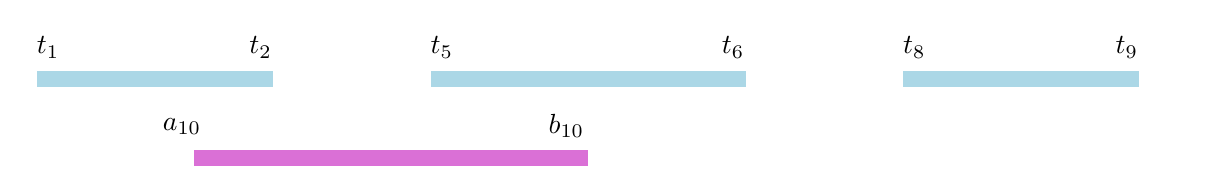
\begin{tikzpicture}

        % \draw [-stealth] (-7,3) -- (-3,3);
        
        \fill [vertexfill] (-7, 2.2) rectangle (-4, 2);
        \fill [vertexfill] (-2, 2.2) rectangle (2, 2);
        \fill [vertexfill] (4, 2.2) rectangle (7, 2);
        
        \fill [Orchid] (-5, 1.2) rectangle (0, 1);
        % \fill [Orchid] (-1.9, 2.9) rectangle (0, 1);
        % \fill [Orchid] (3, 6) rectangle (0, 1);
        

        \node[text width=1cm] at (-6.5,2.5) {$t_1$};
        \node[text width=1cm] at (-3.8,2.5) {$t_2$};
        \node[text width=1cm] at (-1.5,2.5) {$t_5$};
        \node[text width=1cm] at (2.2,2.5) {$t_6$};
        \node[text width=1cm] at (4.5,2.5) {$t_8$};
        \node[text width=1cm] at (7.2,2.5) {$t_9$};
        
        \node[text width=1cm] at (-4.9,1.5) {$a_{10}$};
        \node[text width=1cm] at (0,1.5) {$b_{10}$};
    \end{tikzpicture}
    \caption{The relation of the overlapping relation between $[a_q, b_q]$ and $[t_{im}, t_{jm}]$}
    \label{fig:relation}
\end{figure}
More formally, $u_{qm} = 1$ if the following three conditions hold: (1) $x_{ijm} = 1$, (2) $a_q \leq t_{jm}$, and (3) $t_{im} \leq b_q$. Define a binary decision variable $\alpha_{qijm}$ for every time interval $q \in Q$, every edge $(i, j) \in E^o_e$, and every AV $m \in M^a$ to indicate whether $a_q \leq t_{jm}$. We have $a_q \leq t_{jm}$ if only if $\alpha_{qijm} = 1$. By analogy, we define $\beta_{qijm}$ to indicate whether $t_{im} \leq b_q$.

To capture such sufficient and necessary conditions, we can formulate Constraints \ref{c8} to \ref{c11} for every time interval $q \in Q$ and every vehicle-edge tuple $(m, \; (i,j)) \in S = M^a \times E_e^o$. 
\begin{align}
    &t_{jm} \leq a_q + T\, \alpha_{qijm}, \label{c8}\\
    &t_{jm} \geq a_q + T\, (\alpha_{qijm} - 1), \label{c9} \\
    &b_q \leq t_{im} + T\, \beta_{qijm}, \label{c10} \\
    &b_q \geq  t_{im} + T\, (\beta_{qijm} - 1). \label{c11}
\end{align}

Next, Constraint \ref{c12} is formulated to describe the sufficient condition for $u_{qm} = 1$. 
\begin{equation}
    u_{qm} \geq \frac{1}{3} (\alpha_{qijm} + \beta_{qijm} +x_{ijm}) - \frac{2}{3}, \qquad \forall \; q \in Q, \; \forall \; (m, (i,j)) \in S. \label{c12}
\end{equation}

The last but not least, we count how many remote controllers are occupied by the AV fleet during every time interval and cap it by the budget, which leads to Constraint \ref{c13}.
\begin{equation}
    \sum_{m \in M^a} u_{qm} \leq B, \qquad \forall \; q \in Q. \label{c13}
\end{equation}

The MILP is of polynomial size with respect to the size of the expanded graph and the number of discrete time intervals. The total number of decision variables and the total number of constraints are both $\mathcal{O}(k \; |S| \; |Q|) = \mathcal{O}(k \; |E_e^o| \; |M^a| \; |Q|)$. To summarize, the complete MILP is shown as follows.

\begin{mini}|s|[2]<b>
    {\bm{x}, \bm{y}, \bm{t}, \bm{\alpha}, \bm{\beta}, \bm{u}}
    {RC(\bm{x}) + FC(\bm{y}_o)}{}{}
    \addConstraint{\sum\limits_{j \in \delta^-(i)} x_{ijm}}{ = \sum\limits_{j \in \delta^+(i)} x_{jim} \leq 1, \qquad}{\forall \; i \in V_e - \{o, \; s\}, \; \forall \; m \in M}
    \addConstraint{\sum_{j \in \delta^-(o)} x_{ojm}}{= \sum\limits_{j \in \delta^+(s)} x_{jsm}, \qquad}{\forall \; m \in M}
    \addConstraint{\sum_{i \in D^V(j)} \sum\limits_{m \in M} y_{im}}{= 1, \qquad}{\forall \; j \in D}
    \addConstraint{\sum_{i \in D_e} y_{im} \, d_i}{\leq W, \qquad}{\forall \; m \in M}
    \addConstraint{\sum_{j \in \delta^+(i)} x_{jim}}{\geq y_{im}, \qquad}{\forall \; i \in D_e, \; \forall \; m \in M}
    \addConstraint{X_{ijm}}{ = y_{im}, \qquad}{\forall \; (i, j) \in A, \; \forall \; m \in M}
    \addConstraint{t_{jm}}{\geq t_{im} + \Delta t_{ij} + T \; (x_{ijm} - 1), \qquad}{\forall \; (i, j) \in E_e, \; \forall \; m \in M}
    \addConstraint{T}{\geq t_{sm} = t_{om} + \sum_{(i,j) \in E_e} \Delta t_{ij} x_{ijm}, \qquad}{\forall \; m \in M} 
    \addConstraint{t_{jm}}{\leq a_q + T\, \alpha_{qijm}, \qquad}{\forall \; q \in Q, \; \forall \; (m, (i,j)) \in S}
    \addConstraint{t_{jm}}{\geq a_q + T\, (\alpha_{qijm} - 1), \qquad}{\forall \; q \in Q, \; \forall \; (m, (i,j)) \in S}
    \addConstraint{b_q }{\leq t_{im} + T\, \beta_{qijm}, \qquad}{\forall \; q \in Q, \; \forall \; (m, (i,j)) \in S}
    \addConstraint{b_q }{\geq t_{im} + T\, (\beta_{qijm} - 1), \qquad}{\forall \; q \in Q, \; \forall \; (m, (i,j)) \in S}
    \addConstraint{u_{qm}}{\geq \frac{1}{3} (\alpha_{qijm} + \beta_{qijm} +x_{ijm}) - \frac{2}{3}, \qquad}{\forall \; q \in Q, \; \forall \; (m, (i,j)) \in S}
    \addConstraint{\sum_{m \in M^a} u_{qm}}{\leq B, \qquad}{\forall \; q \in Q}.
\end{mini}

\section{Extended Studies of the MILP} \label{sec:milp_extend}
The MILP proposed in Section \ref{sec:milp}, while exact and polynomial in size, faces limitations when applied to real-world VRP-SA instances. One challenge arises from the discretization of the operational time horizon, which creates a difficult trade-off between model size and performance. Fine granularity leads to a substantial increase in decision variables and constraints, whereas coarse granularity results in holding remote controllers longer than necessary, thereby reducing system capacity. Furthermore, as the system scales, the MILP may quickly become computationally intractable as it is much more complex than typical VRP formulations. In this section, we further explore the MILP formulation from various perspectives, aiming to enhance the model's comprehensiveness and adaptability. The analysis covered will guide the design of a two-phase tractable algorithm discussed in Section \ref{sec:algo}.

\subsection{The Budget Constraint from the Resource Allocation Perspective} \label{resource_allocation}
In the MILP, the time horizon of operation is discretized such that the budget constraint can be enforced at any given moment. In practice, however, the benefit of deploying the AV fleet deteriorates as the granularity of discretization increases, because a time interval may have a long non-overlapping sub-interval (e.g., $[t_2, t_5]$ in Figure \ref{fig:relation}) during which an AV loses the chance to utilize the remote controllers that are indeed available. Therefore, each time interval needs to be short enough. For example, assume the length of time intervals is set to be 30 seconds given that it is a reasonable time for an AV to switch from the automated mode to the remotely-controlled mode, the total number of time intervals in the MILP is as large as 1440 when we have a 12-hour operational window (i.e., $T = 12h$). According to Constraints \ref{c8} to \ref{c13}, the number of variables and constraints in the MILP is multiplied by at least $10^3$ to guarantee a relatively precise time discretization. In this section, we formulate an alternative set of constraints from the perspective of \textit{resource allocation} to meet the real-time budget without time discretization.

We override some notations specified in Table \ref{tab:notations} for a concise representation. Denote by $B$ the set of remote controllers to be allocated. For example, $B$ can be a quad of remote engineers to assist the AV fleet when AVs are on ordinary roads. Let $w = (w^1, w^2) \in E_e^o$ be an AV-enabled edge in the expanded graph, with $w^1$ and $w^2$ representing two end nodes. Define a binary decision variable $u_{bmw}$ for every remote controller $b \in B$, every AV $m \in M^a$, and every edge $w = (i, j) \in E_e^o$. If $u_{bmw} = 1$, the $b$-th unit is assigned to vehicle $m$ while it is on edge $w$. The budget is implicitly satisfied as we only have $|B|$ remote controllers regardless of the assignment. Then, the key idea is to ensure a remote controller $b$ is not assigned to two vehicles simultaneously. More formally, for every two distinct vehicle-edge tuples $(m_1, w_1)$ and $(m_2, w_2)$ in the set $M^a \times E_e^o$ such that $m_1 \neq m_2$, we have $u_{bm_1w_1} + u_{bm_2w_2} \leq 1$ if the following conditions hold:
\begin{enumerate}
    \item Edge $w_1 = (w_1^1, w_1^2)$ is in the route of vehicle $m_1$, which means  $x_{m_1 w_1} = 1$.
    \item Edge $w_2 = (w_2^1, w_2^2)$ is in the route of vehicle $m_2$, which means $x_{m_2 w_2} = 1$.
    \item The time interval of vehicle $m_1$ traversing edge $w_1$ overlaps with the time interval of vehicle $m_2$ traversing edge $w_2$. 
\end{enumerate}
To describe condition 3 rigorously, we further define a binary decision variable $\alpha (w_1, w_2, m_1, m_2)$ for every pair of vehicle-edge tuples in the set $S^2 = \{ ((m_1, w_1), (m_2, w_2)) \; | \; m_1 \neq m_2, \; m_1, m_2 \in M^a, \; w_1, w_2 \in E^o_e\}$. If and only if $\alpha (w_1, w_2, m_1, m_2) = 1$,  the timestamp of vehicle $m_1$ entering edge $w_1$ is earlier than or equal to the timestamp of vehicle $m_2$ exiting edge $w_2$, which means $t_{w_1^1 m_1} \leq t_{w_2^2 m_2}$. By analogy, we define $\beta (w_1, w_2, m_1, m_2)$ to indicate whether the timestamp of vehicle $m_1$ exiting edge $w_1$ is later than or equal to the timestamp of vehicle $m_2$ entering edge $w_2$, namely $t_{w_2^1 m_2} \leq t_{w_1^2 m_1}$. To capture such sufficient and necessary conditions, we can formulate Constraints \ref{c14} to \ref{c17} for every element in $S^2$.
\begin{align}
    &t_{w_2^2 m_2} \leq t_{w_1^1 m_1}+ T\, \alpha (w_1, w_2, m_1, m_2), \label{c14} \\
    &t_{w_2^2 m_2} \geq t_{w_1^1 m_1} + T\, (\alpha (w_1, w_2, m_1, m_2) - 1), \label{c15} \\
    &t_{w_1^2 m_1} \leq t_{w_2^1 m_2} + T\, \beta(w_1, w_2, m_1, m_2), \label{c16} \\
    &t_{w_1^2 m_1} \geq  t_{w_2^1 m_2} + T\, (\beta (w_1, w_2, m_1, m_2) - 1). \label{c17}
\end{align}

Next, for every $b \in B$ and every element in $S^2$, we can formulate Constraint \ref{c18} to describe the sufficient condition for $u_{bm_1w_1} + u_{bm_2w_2} \leq 1$. Finally, the set of Constraints \ref{c14} to \ref{c18} is a replacement for Constraints \ref{c8} to \ref{c13} for a complete MILP. 
\begin{equation}
    u_{bm_1w_1} + u_{bm_2w_2} \leq \frac{11}{4} - \frac{1}{4} (x_{m_1 w_1} + x_{m_2 w_2} + \alpha (w_1, w_2, m_1, m_2) + \beta(w_1, w_2, m_1, m_2)). \label{c18}
\end{equation}

Discarding time discretization is not always beneficial from the complexity point of view. The number of decision variables and the number of constraints in the new MILP are $\mathcal{O}(k \; |S^2| \; |B|)$, which may be more complex than that of the first MILP when the input is a huge road network because $|S^2|$ is $\mathcal{O}(|S|^2)$. In practice, however, we cannot conclude which formulation is superior to the other unless a specific instance is given. 

\subsection{Size Reduction of the MILP} \label{size_reduction}
The MILP proposed in Section \ref{sec:milp} has three folds of extra complexity compared to a basic VRP formulation: (1) The vehicle routing is modeled in a $k$-layer expanded graph. (2) Each layer is a real-world road network instead of the metric closure constructed on the set of customers. (3) A set of constraints, similar to those found in job scheduling problems, is added to the routing component in order to meet the budget of available remote controllers for real-time AV operations. Hence, in this section, we discuss two pre-processing heuristics to reduce the size of the MILP while keeping the sub-optimality gap small in general.

\subsubsection*{Heuristic 1: Reducing the Number of Layers in the Expanded Graph}
In Proposition \ref{prop: k}, we concluded that the number of layers in the expanded graph has to be at least $k$ to guarantee the optimality of the MILP, where $k$ is the maximum number of customers a vehicle can potentially serve under any circumstances and the upper bound of $k$ is the total number of customers in the instance. However, in practice, most urban networks follow a grid-like structure and consist predominantly of two-way roads, which is very different than the pathological example used to prove Lemma \ref{lemma:2}. For more details, refer to Figure \ref{fig:example_network} in Appendix \ref{app: A}. Moreover, the customers and the depot are spatially distributed more uniformly, resulting in less intersecting minimum-cost paths between them. In many of these real-world instances, the chance of a vehicle visiting a single intersection very frequently is significantly reduced. In other words, an optimal vehicle route may pass a single intersection significantly fewer times than $k$. Example \ref{real} illustrates such a realistic instance.
\begin{example} \label{real}
An undirected road network is shown in Figure \ref{fig:real_exp1}. Every node represents an intersection and every edge represents a road segment. The sky-blue node represents the depot and the light-purple nodes represent customers. The routing cost on an edge is proportional to its length. Suppose only one vehicle with unlimited capacity is available in the system. The optimal route can be obtained by observation, which is highlighted in Figure \ref{fig:real_exp2}. Notice that there are 6 customers but only node 2 and node 8 are visited twice. 
\end{example}
\begin{figure}[!htbp]
    \centering
    \begin{subfigure}[b]{0.45\linewidth}
    \centering
    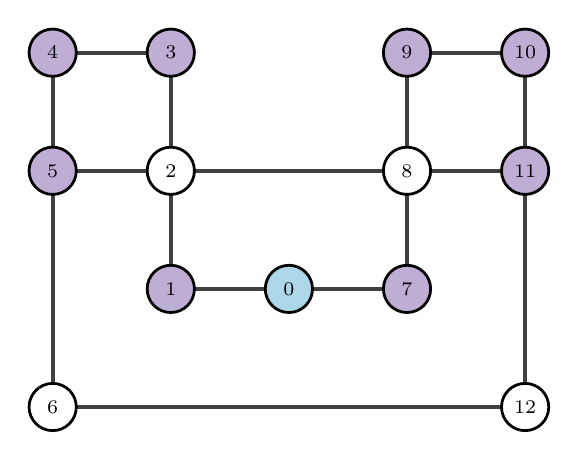
\begin{tikzpicture}

    \Vertex[x = 0, y = 0, label = 0]{0}
    % Left
    \Vertex[x = -1.5, y = 0, RGB, color = {190,174,212}, label = 1]{l1}
    \Vertex[x = -1.5, y = 1.5, color = white, label = 2]{l2}
    \Vertex[x = -1.5, y = 3, RGB, color = {190,174,212}, label = 3]{l3}
    \Vertex[x = -3, y = 3, RGB, color = {190,174,212}, label = 4]{l4}
    \Vertex[x = -3, y = 1.5, RGB, color = {190,174,212}, label = 5]{l5}
    \Vertex[x = -3, y = -1.5, color = white, label = 6]{l6}

    % Right
    \Vertex[x = 1.5, y = 0, RGB, color = {190,174,212}, label = 7]{r1}
    \Vertex[x = 1.5, y = 1.5, color = white, label = 8]{r2}
    \Vertex[x = 1.5, y = 3, RGB, color = {190,174,212}, label = 9]{r3}
    \Vertex[x = 3, y = 3, RGB, color = {190,174,212}, label = 10]{r4}
    \Vertex[x = 3, y = 1.5, RGB, color = {190,174,212}, label = 11]{r5}
    \Vertex[x = 3, y = -1.5, color = white, label = 12]{r6}

    % Left
    \Edge(0)(l1)
    \Edge(l1)(l2)
    \Edge(l2)(l3)
    \Edge(l3)(l4)
    \Edge(l4)(l5)
    \Edge(l5)(l2)
    \Edge(l5)(l6)

    % Reft
    \Edge(0)(r1)
    \Edge(r1)(r2)
    \Edge(r2)(r3)
    \Edge(r3)(r4)
    \Edge(r4)(r5)
    \Edge(r5)(r2)
    \Edge(r5)(r6)

    % Left-Right
    \Edge(l2)(r2)
    \Edge(l6)(r6)
    
    \end{tikzpicture}
    \caption{The road network}
    \label{fig:real_exp1}
    \end{subfigure}
    \hfill
    \begin{subfigure}[b]{0.45\linewidth}
    \centering
    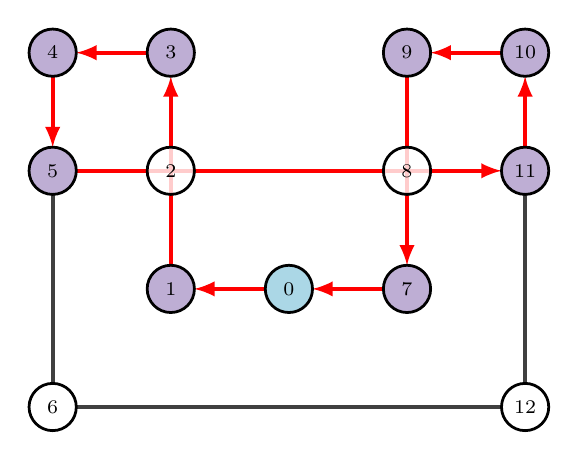
\begin{tikzpicture}

    \Vertex[x = 0, y = 0, label = 0]{0}

    % Left
    \Vertex[x = -1.5, y = 0, RGB, color = {190,174,212}, label = 1]{l1}
    \Vertex[x = -1.5, y = 1.5, color = white, opacity = 0.8, label = 2]{l2}
    \Vertex[x = -1.5, y = 3, RGB, color = {190,174,212}, label = 3]{l3}
    \Vertex[x = -3, y = 3, RGB, color = {190,174,212}, label = 4]{l4}
    \Vertex[x = -3, y = 1.5, RGB, color = {190,174,212}, label = 5]{l5}
    \Vertex[x = -3, y = -1.5, color = white, label = 6]{l6}

    % Right
    \Vertex[x = 1.5, y = 0, RGB, color = {190,174,212}, label = 7]{r1}
    \Vertex[x = 1.5, y = 1.5, color = white, opacity = 0.8, label = 8]{r2}
    \Vertex[x = 1.5, y = 3, RGB, color = {190,174,212}, label = 9]{r3}
    \Vertex[x = 3, y = 3, RGB, color = {190,174,212}, label = 10]{r4}
    \Vertex[x = 3, y = 1.5, RGB, color = {190,174,212}, label = 11]{r5}
    \Vertex[x = 3, y = -1.5, color = white, label = 12]{r6}

    % Left
    \Edge[Direct, color = red](0)(l1)
    \Edge[Direct, color = red](l1)(l3)
    % \Edge[Direct, color = red](l2)(l4)
    \Edge[Direct, color = red](l3)(l4)
    \Edge[Direct, color = red](l4)(l5)
    % \Edge[Direct, color = red](l5)(l2)
    \Edge(l5)(l6)

    % Reft
    \Edge[Direct, color = red](r1)(0)
    % \Edge[Direct, color = red](r2)(r1)
    \Edge[Direct, color = red](r3)(r1)
    \Edge[Direct, color = red](r4)(r3)
    \Edge[Direct, color = red](r5)(r4)
    % \Edge[Direct, color = red](r2)(r5)
    \Edge(r5)(r6)

    % Left-Right
    \Edge[Direct, color = red](l5)(r5)
    \Edge(l6)(r6)
    % \Edge[Direct, path = [0, l1, l2, l3, l4, l5, l2, r2, r5, r4, r3, r2, r1, 0]]{}{}
    
    \end{tikzpicture}
    \caption{The optimal route}
    \label{fig:real_exp2}
    \end{subfigure}
    \caption{A realistic VRP instance in the real-world road network}
\end{figure}

Hence, it is justified to reduce the number of layers in the expanded graph from $k$ to a smaller integer $\overline{k}$. Nevertheless, a naive reduction may cause a highly sub-optimal solution or even make the MILP infeasible because the transition Constraint \ref{c5} forces every vehicle to move one layer up every time it serves a customer except that it is already on the topmost layer. When $\overline{k} << k$, any vehicle tends to move to the topmost layer as soon as possible even though the route does not intersect with itself in serving the first few customers. In Example \ref{real}, a 3-layer expanded graph is sufficient as no node is visited more than twice in the optimal solution shown in Figure \ref{fig:real_exp2}, but the existence of Constraint \ref{c5} excludes this true optimal solution from the feasible space, resulting in a sub-optimal solution that re-routes to edge $(5, 6)$ instead of edge $(5, 2)$.

To circumvent this disadvantage, we re-design the transition constraint by replacing Constraint \ref{c5} with Constraint \ref{transition}. Due to the inequality, a transition of layers after serving a customer is no longer compulsory but optional. The transition only occurs if it leads to a better solution. Despite the improvement by this soft transition constraint, an ``optimal'' solution given by the updated MILP can still deviate from a true optimum of the problem if $\overline{k}$ is too small for a given instance. One strategy is to solve the MILP with $\overline{k} = 1$ and iteratively increase $\overline{k}$ until the optimal value converges or the reduced cost is less than a small threshold.  
\begin{align}
    x_{ijm} \leq y_{im}, \qquad \forall \; (i, j) \in A, \; \forall \; m \in M. \label{transition}
\end{align}

\subsubsection*{Heuristic 2: Pre-Prune the Road Network}
The network pre-pruning heuristic is motivated by Proposition \ref{pruning} presented in the work by Rodriguez-Pereira et al. \cite{RODRIGUEZPEREIRA2019615}. Recall that the VRP-SA generalizes from the STSP, where both the depot and customers are regarded as required nodes. Intuitively, if an edge is part of an optimal solution to a VRP-SA instance, it is highly probable to appear in a minimum-cost path between customers or in a path that utilizes remote controllers for the least amount of time. Therefore, it is justifiable to pre-prune the input road network before we construct the expanded graph.

The pre-processing steps are as follows: (1) Compute the minimum-cost paths between any pair of nodes in the set of customers and the depot. Denote by $P_1$ and $V_1$ the set of all edges and nodes used in those paths, respectively. (2) Compute the paths for any pair of nodes in the set of customers and the depot such that each path utilizes remote controllers for the shortest duration. Denote by $P_2$ and $V_2$ the set of edges and nodes used in those paths, respectively. (3) Identify all other AV-enabled strongly connected components that are connected to $P_1$ and $P_2$. Denote by $P_3$ and $V_3$ the set of all edges and nodes used in such components, respectively. (4) Remove all edges that are not in $P_1 \cup P_2 \cup P_3$ and all nodes that are not in $V_1 \cup V_2 \cup V_3$. The resulting sparse subgraph $G_s = (V_1 \cup V_2 \cup V_3, \; P_1 \cup P_2 \cup P_3)$ replaces the original network $G$ and is used to construct the expanded graph $G_e$. 
\begin{proposition} \label{pruning}
In any optimal solution to a given Steiner traveling salesmen problem instance, all edges used belong to some minimum-cost paths in the network connecting two required nodes. 
\end{proposition}


\section{A Two-Phase Tractable Algorithm} \label{sec:algo}
As discussed in Section \ref{size_reduction}, the size complexity of the original MILP renders it computationally intractable for any practical instances in the real world. Even with the application of the aforementioned size reduction heuristics in Section \ref{size_reduction}, directly solving the VRP-SA using the most powerful MILP solver remains challenging. Therefore, in this section, we develop a two-phase algorithm to efficiently find high-quality solutions to medium-size VRP-SA instances with up to 100 customers and 2000 edges in the road network. 

In phase 1, given any instance $\mathcal{I}_0$ of the VRP-SA, we create an instance $\mathcal{I}_1$ of the \textit{Heterogeneous Vehicle Routing Problem with Fixed Costs and Vehicle-Dependent Routing Cost (H-VRP-FD)} by removing the budget constraint of remote controllers. Naturally, the optimal value of $\mathcal{I}_1$ is a lower bound for that of $\mathcal{I}_0$. Then, we solve $\mathcal{I}_1$ efficiently to obtain a near-optimal solution. The exact optimum can be also pursued if the instance size permits. Currently, the state-of-the-art exact and heuristic approaches for this VRP variant are due to Baldacci and Mingozzi \cite{baldacci2009unified} and Vidal et al. \cite{VIDAL2014658}, respectively.

By decoding the solution to $\mathcal{I}_1$, we can derive all routes of vehicles dispatched. Denote by $\Tilde{X}$ the set of routes of the HDV fleet, and by $X$ the set of routes of the AV fleet. In particular, $\Tilde{X} = \{X(m) \; | \; \forall \; m \in \overline{M}^h\}$ and $X = \{X(m) \; | \; \forall \; m \in \overline{M}^a\}$, where $X(m)$ is the \textit{route} of vehicle $m$ represented as a sequence of road intersections visited, and $\overline{M}^h$ ($\overline{M}^a$) is the set of all dispatched (HDVs) AVs. Each $X(m)$ can be used to infer the \textit{routing schedule} $\mathcal{T}(m)$, which contains the timestamps of the vehicle visiting intersections on the route. All vehicle departure times are set to be zero. Denote by $\Tilde{\mathcal{T}} = \{\mathcal{T}(m) \; | \; m \in \overline{M}^h\}$ the set of routing schedules of dispatched HDVs, and by $\mathcal{T} = \{\mathcal{T}(m) \; | \; m \in \overline{M}^a\}$ the set of routing schedules of dispatched AVs. 

In phase 2, we check whether the set of routing schedules $\mathcal{T}$ is feasible with respect to the budget of remote controllers, and recover the solution feasibility if necessary. Recall that $\Tilde{\mathcal{T}}$ does not impact the feasibility of the solution to $\mathcal{I}_0$ since HDVs do not require assistance from remote controllers. However, the schedules $\mathcal{T}$ for AVs might be infeasible. For any two consecutive timestamps, $t_{im}$ and $t_{jm}$, in the routing schedule $\mathcal{T}(m)$, we can determine whether AV $m$ occupies a remote controller depending on the type of edge $(i, j)$. This enables us to efficiently verify whether $(X, \; \mathcal{T})$ violates the budget constraint over certain time intervals. If the budget is not exceeded, then $(\Tilde{X} \cup X, \; \Tilde{\mathcal{T}} \cup \mathcal{T})$ is a feasible and therefore an optimal solution to $\mathcal{I}_0$. On the contrary, if the budget is exceeded, we solve a \textit{feasibility recovering sub-problem (FRP)} to find a near-optimal solution $(\Tilde{X} \cup X^*, \;  \Tilde{\mathcal{T}} \cup \mathcal{T}^*
)$ to $\mathcal{I}_0$, where $(X^*, \; \mathcal{T}^*)$ are the updated AV routes and their schedules. Two families of FRP based on \textit{re-scheduling} strategy and \textit{re-routing} strategy will be discussed in Section \ref{sec:frp1} and Section \ref{sec:frp2}, respectively.

The two-phase algorithmic pipeline is detailed in Algorithm \ref{algo:holistic}, with the sub-routines in Line 3 and Line 6 elaborated later. It is important to note that neither the re-scheduling FRP nor re-routing FRP guarantees a complete recovery of the solution feasibility for $(\mathcal{X}, \mathcal{T})$. In the worst case, it may be necessary to replace some AVs with HDVs to serve certain customers and avoid exceeding the budget. If no additional HDVs are available in the system, the instance will be deemed infeasible.
\begin{algorithm}[!htbp]
\caption{The Two-Phase Algorithmic Pipeline to Solve the VRP-SA}

\begin{algorithmic}[1]
\Require A VRP-SA instance $\mathcal{I}_0$
\Ensure Feasible vehicle routes are schedules $(\Tilde{X} \cup X^*, \; \Tilde{\mathcal{T}} \cup \mathcal{T}^*)$

\State Construct an instance $\mathcal{I}_1$ of the H-VRP-FD based on $\mathcal{I}_0$, 
\State $(\Tilde{X}, \; X, \; \Tilde{\mathcal{T}}, \; \mathcal{T}) \gets \texttt{HVRPPDSolver} (\mathcal{I}_1)$ 
% \State $(\Tilde{\mathcal{T}}, \; \mathcal{T}) \gets \texttt{ExtractSchedules}(\Tilde{X}, \; X)$
\State $\mathcal{T}^* \gets \texttt{ReSchedulingFRPSolver}(\mathcal{T})$
\State $X^* \gets X$
\If{$\mathcal{T}^* = \varnothing$}
\State $(\overline{D}, \; X^*, \; \mathcal{T}^*) \gets \texttt{ReRoutingFRPSolver}(X, \; \mathcal{T})$
\If{ $\overline{D} \neq \varnothing$}
\State $\Tilde{X}_{\overline{D}} \gets \texttt{CVRPSolver}(\overline{D})$
\State $\Tilde{X} \gets \Tilde{X} \cup \Tilde{X}_{\overline{D}}$
\EndIf
\EndIf
\end{algorithmic}
 \label{algo:holistic}
\end{algorithm}

Theoretically, Algorithm \ref{algo:holistic} may still fail to return a feasible solution even though $\mathcal{I}_0$ is indeed feasible. This limitation stems from the inherent nature of the relax-then-recover framework, which decomposes customer assignment and sequencing without incorporating a mechanism to iteratively explore the entire search space of the VRP-SA. Consequently, it may miss feasible solutions that require more nuanced exploration. However, we hypothesize that, under realistic conditions in the real world, a VRP-SA instance is very likely to be infeasible if Algorithm \ref{algo:holistic} fails to find a feasible solution.

\subsection{The Re-Scheduling Feasibility Recovering Sub-Problem} \label{sec:frp1}
One strategy to recover the feasibility of $(X, \; \mathcal{T})$ is to re-schedule $\mathcal{T}$ while keeping the set of routes $X$ unchanged. For each routing schedule $\mathcal{T}(m)$, we can extract a subset of timestamps called \textit{transition timestamps}, at which an AV switches between an AV-enabled road and an ordinary road. All road segments of the same type traveled between any two consecutive transition timestamps can be merged into a \textit{sub-route}. We observe that, the departure time is not necessarily zero for every vehicle in the optimal solution to the VRP-SA, as the departure delay of some vehicles may benefit the system by adding more feasibility to the temporal space of the problem. In another word, the routing schedule of every AV, as a whole, can potentially be shifted forward in time to avoid budget violations, provided the vehicle’s return time is earlier than the end of the operation horizon $T$.

Figure \ref{fig:frp1} illustrates this re-scheduling process for a small instance with two AVs and a single remote controller. In the figure, each strip represents a time interval during which an AV occupies a remote controller on an ordinary sub-route. The original schedules are infeasible due to overlapping strips between vehicles $m_1$ and $m_2$. If we delay the departure of vehicle $m_2$ by $\delta$, highlighted in purple strips, the schedules become feasible. This rescheduling does not increase the overall cost, as a departure delay does not inherently affect the operation negatively. In general, the \textit{re-scheduling FRP} takes $\mathcal{T}$ as the input and aims to find a feasible shift of the routing schedule $\mathcal{T}(m)$ for every dispatched vehicle $m$, such that the updated schedules $\mathcal{T}^*$ are feasible to $\mathcal{I}_0$.
\input{figures/re-scheduling-visualization}

The re-scheduling FRP is a feasibility problem that can be exactly modeled by an MILP without an objective function, referred to as the \textit{re-scheduling MILP}, which will be elaborated upon later. Notably, the formulation of this re-scheduling MILP resembles the constraints in Section \ref{resource_allocation} which handled the budget constraint from a resource allocation perspective.

Denote by $R = R^a \cup R^o$ the set of sub-routes, where $R^a$ is the subset of AV-enabled sub-routes and $R^o$ is the subset of ordinary sub-routes. Denote by $\Delta t_r$ the travel time in sub-route $r$. Define a continuous decision variable $\overline{t}_m \in  [0, T]$ as the re-scheduled departure time for each dispatched AV $m \in \overline{M}^a$. Furthermore, define two continuous decision variables $t^1_r \in [0, T]$ and $t^2_r \in [0, T]$ as the timestamp of the associated vehicle entering and exiting sub-route $r$, respectively. Then, the consistency among timestamps can be captured by Constraints \ref{frp1:c1} and \ref{frp1:c2}, where $r' \prec r$ means sub-route $r'$ is traversed earlier than sub-route $r$ on the same route. 
\begin{align} 
    &t_r^1 = \overline{t}_m + \sum_{r': \; r' \prec \, r} \Delta t_{r'}, \qquad \forall \; r \in R, \label{frp1:c1} \\
    &t_r^2 = t_r^1 + \Delta t_r, \qquad \forall \; r \in R. \label{frp1:c2}
\end{align}

Define a binary variable $u_{br} \in \{0, 1\}$ for every remote controller $b \in B$ and every ordinary sub-route $r \in R^o$. If $u_{br} = 1$, the $b$-th controller is assigned to the sub-route $r$. Constraint \ref{frp1:extra} regulates the unique assignment of one remote controller to a single ordinary sub-route.
\begin{gather}
    \sum_{b \in B} u_{br} = 1, \qquad \forall \; r \in R^o.
    \label{frp1:extra}
\end{gather}

Define a set $R^2 = \{(r_1, r_2) \; | \; r_1, r_2 \in R^o, \; r_1 \nparallel r_2\}$, where $r_1 \nparallel r_2$ means sub-routes $r_1$ and $r_2$ are not on the same route. For each pair of sub-routes in $R^2$, define a binary decision variable $\alpha(r_1, r_2)$. If and only if $\alpha(r_1, r_2) = 1$, the start time of sub-route $r_1$ is earlier than or equal to the end time of sub-route $r_2$, which means $t_{r_1}^1 \leq t_{r_2}^2$. By analogy, we define $\beta (r_1, r_2)$ to indicate whether the the end time of sub-route $r_1$ is later than or equal to the start time of sub-route $r_2$, namely $t_{r_2}^1 \leq t_{r_1}^2$. To capture these sufficient and necessary conditions, we formulate Constraints \ref{frp1:c3} to \ref{frp1:c6}.
\begin{align}
    &t_{r_2}^2 \leq t_{r_1}^1 + T \; \alpha(r_1, r_2), \qquad \forall \; (r_1, r_2) \in R^2,\label{frp1:c3} \\
    &t_{r_2}^2 \geq t_{r_1}^1 + T \; (\alpha(r_1, r_2) - 1),  \qquad \forall \; (r_1, r_2) \in R^2, \label{frp1:c4} \\
    &t_{r_1}^2 \leq t_{r_2}^1 + T \; \beta(r_1, r_2), \qquad \forall \; (r_1, r_2) \in R^2, \label{frp1:c5} \\
    &t_{r_1}^2 \geq t_{r_2}^1 + T \; (\beta(r_1, r_2) - 1),  \qquad \forall \; (r_1, r_2) \in R^2. \label{frp1:c6}
\end{align}

Then, we can formulate Constraint \ref{frp1:c7} to avoid a remote controller being assigned to two ordinary sub-routes simultaneously. Overall, all the constraints of the re-scheduling MILP are listed from \ref{frp1:c1} to \ref{frp1:c7}.
\begin{gather}
    u_{br_1} + u_{br_2} \leq \frac{5}{2} - \frac{1}{2} (\alpha(r_1, r_2) + \beta(r_1, r_2)), \qquad \forall \; (r_1, r_2) \in R^2. \label{frp1:c7}
\end{gather}

One may notice that the re-scheduling FRP is also an NP-hard problem, and the core constraints from \ref{frp1:c3} to \ref{frp1:c7} in the re-scheduling MILP exhibit structural similarity to the highly complex constraints discussed in Section \ref{resource_allocation}. In practice, however, the re-scheduling FRP can be solved much more efficiently as the total number of sub-routes is much less than the total number of edges in the network. It is justified because AV-enabled roads tend to form a skeleton within the network as smart infrastructure develops, leading to less frequent transitions between AV-enabled road segments and ordinary road segments along a vehicle route. 

Building on the concept of flexible departure times aforementioned, we further explore a scenario where the travel times of AVs on each road segment is also flexible. This unlocks an even larger feasible space for both the VRP-SA and the re-scheduling FRP. Detailed discussions are provided in Appendix \ref{Appendix B}.

\subsection{The Re-Routing Feasibility Recovering Sub-Problem} \label{sec:frp2}
In this section, we discuss the re-routing strategy to recover the feasibility of $(X, \mathcal{T})$. Unlike the re-scheduling FRP, the re-routing FRP takes both $X$ and $\mathcal{T}$ as the input and aims to find a feasible set of vehicle routes $X^*$ along with the updated routing schedules $\mathcal{T}^*$. Importantly, the customer-to-vehicle assignment remains unchanged, with adjustments made only within individual vehicle routes.

The re-routing FRP is an optimization problem with the objective of minimizing the additional cost incurred by route perturbation. It generalizes the re-scheduling FRP, as perturbing a route includes the special case of adjusting only the departure time (or all timestamps under the flexible travel time assumption discussed in Appendix \ref{Appendix B}). Due to its complexity, finding an exact solution is challenging. Therefore, we develop an iterative algorithm based on the \textit{ruin-and-recreate} principle and a \textit{route priority heuristic} to solve it approximately. 

First of all, we convert $(X, \mathcal{T})$ to a priority queue, where the priority of a route $X(m)$ is determined by its value $v(m)$, as defined in Equation \ref{eq:heuristic}. Two cost adjustment factors $\eta_1 < 1$ and $\eta_2 > 1$ that are defined in Section \ref{sec:description} play a key role here. Let $c^1(m)$ and $c^2(m)$ represent the total routing costs of AV-enabled roads and ordinary roads, respectively, in route $X(m)$. Routes that better utilize AV-enabled roads are more valuable compared to HDV routes. We also initialize $X^{*}$ and $\mathcal{T}^{*}$ as two empty containers to store feasible routes and their routing schedules.
\begin{equation} \label{eq:heuristic}
    v(m) = \frac{1 - \eta_1}{\eta_1} \; c^1 (m) + \frac{1 - \eta_2}{\eta_2} \; c^2(m)
\end{equation}

Then, in each iteration, the algorithm pops the route $X(m)$ with the highest value from the priority queue and examines whether its routing schedule $\mathcal{T}(m)$, when combined with any other existing routing schedules in $\mathcal{T}^{*}$, violates the budget constraint at a certain point in time. If no violation occurs, $X(m)$ and $\mathcal{T}(m)$ are moved to the feasible containers, and the algorithm proceeds to the next iteration. If a violation is detected, the current route $X(m)$ is ``ruined'', and the algorithm attempts to recreate a new route $X^*(m)$ such that the following two constraints are satisfied: (1) Vehicle $m$ avoids ordinary road segments when the budget is exhausted or exceeded given the schedules of remaining routes. (2) The return time of vehicle $m$ is less than the end time of operation. The re-creation process is essentially solving a \textit{Constrained Steiner Traveling Salesman Problem} (CSTSP). It takes as input the original network $G$, the subset of customers $D(m)$ served by the current route $X(m)$, the operational end time $T$, and the feasible routing schedules $\mathcal{T}^{*}$, and output a new feasible route $X^*(m)$ or report that no solution exists. Whenever the algorithm fails to recreate a feasible route cheaper than dispatching an HDV, it adds $D(m)$ to the set of unserved customers $\overline{D}$. 

The CSTSP, a crucial component of the algorithm, can be modeled similarly to the VRP-SA discussed in Section \ref{sec:milp}, but with substantially reduced complexity. We first apply the size reduction heuristics from Section \ref{size_reduction} and construct an expanded graph $G_e(m)$ following the steps in Section \ref{sec:milp}. The resulting graph is considerably smaller than $G_e$ for the full VRP-SA because the graph pre-pruning removes more edges given that $|D(m)| < |D|$. We then formulate a similar MILP, called \textit{re-routing MILP}, based on $G_e(m)$. The primary modifications are highlighted as follows while further details are provided in Appendix \ref{Appendix C}.
\begin{enumerate}
    \item Since the problem involves only one vehicle route, which must be dispatched, we eliminate the fixed cost component from the objective function and remove the vehicle index from all decision variables.
    \item Manual time discretization is unnecessary. Instead, we construct the set of non-overlapping time intervals by partitioning the operational time horizon $[0, T]$ based on the timestamps in the set $\{(i, j) \; | \; i, j \in \mathcal{T}' \cup \{T\}\}$, where $\mathcal{T}' = \bigcup_{\mathcal{T}(m) \in \mathcal{T}^{*}} \mathcal{T}(m)$ represents a merged set of timestamps from the current feasible routing schedules $\mathcal{T}^{*}$. 
\end{enumerate}

\begin{algorithm}[!t]
\caption{The re-routing FRP solver}
\begin{algorithmic}[1]
\Require Graph $G$, AV routes and schedules $(X, \; \mathcal{T})$, End time of operation $T$
\Ensure Updated AV routes and schedules $(X^*, \; \mathcal{T}^*)$, Unserved customers $\overline{D}$

\State $(X, \; \mathcal{T}) \gets \texttt{PriorityQueueByValues}(X, \; \mathcal{T})$
\State Initialize $(X^*, \mathcal{T}^*) = (\varnothing, \varnothing)$

\While{$(X, \mathcal{T}) \neq \varnothing$}
% \For{$(X(m), \mathcal{T}(m))$ in $(X^*, \mathcal{T}^*)$}

\State $(X(m), \mathcal{T}(m)) \gets (X, \mathcal{T}).\texttt{dequeue()}$

\If{$\mathcal{T}^{*} \cup \{\mathcal{T}(m)\}$ does not violate budget at any time}
\State $X^* \gets X^* \cup \{X(m)\}$
\State $\mathcal{T}^* \gets \mathcal{T}^* \cup \{\mathcal{T}(m)\}$
\State \textbf{continue}
\EndIf

\State $D(m) \gets \texttt{ExtractCustomers}(X(m))$
\State $G_s(m) \gets \texttt{GraphPruner}(G, D(m))$
\State $G_e(m) \gets \texttt{GraphExpander}(G_s(m))$
\State $(X^*(m), \; \mathcal{T}^*(m)) \gets \texttt{ReRoutingMILPSolver}(G_e(m), \; D(m), \; \mathcal{T}^*, \; T)$
\State $UB \gets \texttt{TSPSolver}(D(m))$
\If{$X^*(m) = \varnothing$ or $X^*(m)$ is more expansive than $UB$}
\State $\overline{D} \gets \overline{D} \cup D(m)$
\Else
\State $X^* \gets X^* \cup \{X^*(m)\}$
\State $\mathcal{T}^* \gets \mathcal{T}^* \cup \{\mathcal{T}^*(m)\}$
\EndIf
% \EndFor
\EndWhile
\end{algorithmic}
\label{algo:re-routing-frp}

\end{algorithm}

Overall, Algorithm \ref{algo:re-routing-frp} provides a complete pseudo-code for the re-routing FRP solver. As aforementioned, the order of iteration of routes is not arbitrary but depends on the route priority heuristic. Routes with higher values are less likely to be perturbed or replaced, which guides the algorithm towards solutions with lower total routing costs. Additionally, if the algorithm terminates with a non-empty set $\overline{D}$, it indicates that the feasibility of $(X, \mathcal{T})$ has not been fully recovered. This outcome could be due to one of the following reasons: (1) the re-routing FRP is infeasible with the current customer-to-vehicle assignments, or (2) the re-routing FRP is feasible but the algorithm fails to find a feasible solution. Nevertheless, the algorithm is devised to recover the feasibility to the greatest extent possible.

\section{Numerical Experiments} \label{sec:exp}
% \Hins{The experiments are re-running to account for the change of unit routing cost for AVs on ordinary roads.}
In this section, we construct a tailored set of instances for the VRP-SA and solve them using Algorithm \ref{algo:holistic} described in Section \ref{sec:algo}. The results (1) validate the effectiveness and efficiency of the proposed two-phase algorithm and (2) illustrate how variations in input parameters influence both the problem structure and the corresponding solutions.

\subsection{VRP-SA Instances} \label{instances}
We construct 23 VRP-SA instances, each based on a CVRP instance from the benchmark dataset P described by Augerat \cite{augerat1995computational}. The number of customers in these CVRP instances ranges from 16 to 101. Each CVRP instance provides the following inputs: the coordinates of the depot and customers in a 2D Euclidean space, customer demands, and a uniform vehicle capacity. These inputs are directly adopted for the corresponding VRP-SA instances.

To accommodate the additional attributes of the VRP-SA, we construct an underlying road network for each CVRP instance based on the coordinates of all nodes. The process is as follows: (1) Draw a rectangular bounding box such that the farthest nodes are positioned along its boundary. (2) Construct a primary grid by equally dividing the bounding box along both the x- and y-axes, with two hyperparameters, $g_x$ and $g_y$, determining the number of divisions in each direction. Unless otherwise specified, we set $g_x = g_y = 5$ in the following experiments. This grid serves as the skeleton of the underlying road network, where all road segments are AV-enabled. (3) Within each cell of the primary grid, we construct a local grid, where each customer within the cell is placed precisely at an intersection. All road segments within the local grids are ordinary roads. Figure \ref{fig:network} illustrates the underlying road network of instance P-n40-k5. The design aims to mimic real-world semi-autonomous environments, where infrastructure upgrades to support AVs are prioritized on primary avenues in cities.  
\begin{figure}[!htbp]
    \centering
    \includegraphics[width=0.8\linewidth]{network-2.png}
    \caption{The underlying road network of P-n40-k5}
    \label{fig:network}
\end{figure}

As assumed in Section \ref{sec:description}, the unit routing cost of an AV on the primary grid is lower than that of an HDV. Conversely, it is more cost-demanding for an AV to travel on local grids than an HDV. For HDVs, the routing cost on any edge in the road network is equal to the edge length. For AVs, the routing cost on an edge in the primary grid is given by $\eta_1$ times the edge length, while on local grids, it is $\eta_2$ times the edge length. In the following experiments, we set $\eta_1 = 0.5$ and $\eta_2 = 1.2$ if not otherwise specified. 

To guarantee that all VRP-SA instances are feasible, which simplifies the analysis of experimental results, we set the size of the AV fleet, $|M^a|$, and the HDV fleet, $|M^h|$, in each VRP-SA instance to match the number of vehicles used in the optimal solution of the corresponding CVRP instance. To avoid over-dispatching, we assign an equal fixed dispatch cost (e.g., 1) to all vehicles.

For each VRP-SA instance, we define the operation end time as $T = T_{factor} \cdot \overline{T}$, where $\overline{T}$ is the maximum return time of all vehicles in the optimal solution to the CVRP instance with only HDVs deployed. The parameter $T_{factor} \in [1, \infty]$ serves as a time-horizon factor that controls the relative tightness of the operation time window. Note that travel time and routing cost are used interchangeably since the VRP instances in this section are synthetic. In the following experiments, we set $T_{factor} = 1.2$, unless otherwise specified.

Finally, we introduce a budget $B$ that determines the number of remote controllers available to assist AVs on ordinary local grids. In the experiments, we set $B = \max(1, \; \texttt{round}(\frac{|M^a|}{3}))$ unless otherwise specified, which roughly corresponds to one-third of the AV fleet size in each VRP-SA instance. This percentage-based approach provides more flexibility, as the minimum number of dispatched vehicles varies significantly across instances. 

\subsection{Algorithm Settings} \label{setting}
Strictly speaking, the algorithm must solve an H-VRP-PD in Phase 1, as shown in Line 2 of Algorithm \ref{algo:holistic}, before proceeding to Phase 2 for re-scheduling or re-routing. This initial step is computationally intensive. From an experimental standpoint, we simplify Phase 1 by solving a CVRP with only the AV fleet deployed, under the same settings. While this solution is suboptimal compared to that for the H-VRP-PD, it reduces computational demands. In practice, the algorithm’s performance can be further improved by exactly solving the H-VRP-PD, which would provide a true lower bound for the VRP-SA. For the CVRP, we use the state-of-the-art solver \textit{HGS-CVRP} developed by Vidal \cite{VIDAL2022105643}. The TSP solver used in Line 14 of Algorithm \ref{algo:re-routing-frp} is from Google OR-Tools. All other MILPs are solved using Gurobi 10.0.1, with several hyperparameters fine-tuned for each instance. Specifically, the \texttt{TimeLimit} for all Gurobi solvers is set to 300 seconds to enforce termination. Unless otherwise specified, the number of layers $k$ in the expanded graph is set to 2.

\subsection{Baseline Results} \label{result}
For each VRP-SA instance, we denote $f^P$ as the routing cost obtained using the proposed algorithm with the re-routing priority heuristic, and $f^{\overline{P}}$ as the routing cost obtained with a random re-routing order. Additionally, we denote $f_1$ as the near-optimal routing cost for the CVRP instance with only the AV fleet deployed, as obtained in Phase 1, and $f_2$ as the near-optimal routing cost for the CVRP instance with only the HDV fleet deployed, representing the cost without exploiting AVs at all. To account for variability due to instance sizes, we report the \textit{routing cost ratios} $f_2 / f_1$, $f^P / f_1$, and $f^{\overline{P}} / f_1$, instead of the absolute routing costs, for all instances ranging from 0 to 22. Given an instance, the quantity $f_2 / f_1 - 1$ approximately measures the percentage increase in routing cost when operating in a non-autonomous environment compared to a semi-autonomous environment with unlimited remote controllers. Similarly, $f^P / f_1 - 1$ or $f^{\overline{P}} / f_1 - 1$ quantify the percentage increase in routing cost under a limited budget of remote controllers.
\begin{figure}[!htbp]
    \centering
    \includegraphics[width = 0.9\linewidth]{main_result.png}
    \caption{Routing cost ratios in different VRP-SA instances}
    \label{fig:main_result}
\end{figure}

As shown in Figure \ref{fig:main_result}, the proposed algorithm with only a random re-routing order generally yields lower routing cost ratios than the baseline with only the HDV fleet deployed (i.e., no AVs involved), except for instance 20. The greatest cost reduction is over 37.5\% in instance 5. If the re-routing priority heuristic is enabled, the algorithm performs even better in most cases, except for instance 22. Moreover, the algorithm successfully re-schedules the vehicle routes obtained in Phase 1 to feasibility without evoking the re-routing component in 8 out of 23 instances (i.e., instances 0, 1, 5, 6, 7, 10, 11, and 14), which is advantageous as it results in zero additional routing cost. More numerical details are available in Appendix \ref{Appendix C}.

We also observe two secondary patterns from the results: (1) As instance size increases, $f_2 / f_1$ tends to decrease. Since the instances in Figure \ref{fig:main_result} are ordered first by the number of customers and then by the number of available vehicles, this trend is expected. The number of divisions, $g_x$ and $g_y$, in the primary grid remains fixed across all instances, leading to a higher customer density within each grid cell for larger instances. Consequently, AV-enabled roads become relatively ``sparser'' in larger instances, diminishing the advantage of dispatching AVs. The effect of AV-enabled road density is further examined in Section \ref{heatmap}. (2) In instances where $f_2 / f_1$ is relatively low (e.g., instances 2, 3, 4, 8, 9, 13, and 16), $f^{\overline{P}} / f_1$ or $f^P / f_1$ tend to be relatively high, and vice versa. This pattern follows a similar rationale as the first. When $f_2 / f_1$ is low, AVs face greater difficulty in effectively leveraging AV-enabled roads, making re-routing less feasible and increasing its cost.

\subsection{Sensitivity Analysis of Input Parameters} \label{heatmap}
We conduct a series of experiments by varying the budgets and time-horizon factors while keeping other input parameters at their default values. Specifically, we set $B = \max(2, \; \texttt{round}(|M^a| \cdot B_{factor}))$ with $B_{factor} = (1/3, \; 1/2, \; 2/3)$ and $T_{factor} = (1.0, \; 1.1, \; 1.2, \; 1.3, \; 1.4, \; 1.5)$. The results shown in Figure \ref{fig:H1} and Figure \ref{fig:H2} are the average values across all 23 instances. As the budget and the tightness of the operational time horizon increase, the routing cost ratio $f^P / f_1$ decreases to as low as 1.006, resulting in a significant cost reduction of up to 22\%. Theoretically, an instance with a looser time-horizon factor should save more cost than that with a tighter time-horizon factor. The observed discrepancy for the results of $(B_{factor}, \; T_{factor}) = (1/2, \; 1.4)$ is attributed to the indeterministic behavior in the Gurobi solver under the parameter setting concerning the maximum running time.
\begin{figure}[!htbp]
    \centering
    \begin{subfigure}[t]{0.49\linewidth}
    \centering
    \includegraphics[width = \linewidth]{real_H1_heuristic.png}
    \caption{Average routing cost ratios $f^P / f^1$}
    \label{fig:H1}
    \end{subfigure}
    \begin{subfigure}[t]{0.49\linewidth}
    \centering
    \includegraphics[width = \linewidth]{real_H2_heuristic.png}
    \caption{Average cost reduction due to VRP-SA}
    \label{fig:H2}
    \end{subfigure}
    \caption{Changing budget and the tightness of operational time horizon}
\end{figure}

We also vary the number of divisions $g_x$ and $g_y$ from 3 to 7 in the primary grid, while keeping other input parameters at their default values. Figure \ref{fig:grid_size} shows the \textit{inverse routing cost ratio} $f_1 / f_2$, where the ratio upper bound is 1.0, representing the cost of dispatching only HDVs. According to the result, it becomes increasingly advantageous to replace HDVs with AVs in networks with denser AV-enabled roads. Moreover, ratio $f^P / f_2$ closely follows the trend of $f_1/ f_2$, indicating that the proposed model and algorithm effectively leverage the increased density of AV-enabled roads to reduce routing costs. The density of AV-enabled roads serves as a metric for quantifying the degree of transition from a current environment to a fully autonomous one. Interestingly, the results reveal a two-stage pattern in this trend. In stage one (i.e., $g_x = g_y \leq 5$) when the density is relatively low, the gap between $f^P / f_1$ and $f_1 / f_2$ widens as the density increases. This is due to the budget constraint of remote controllers, which limits AVs from using all available road segments in routing. In stage two (i.e., $g_x = g_y \geq 5$) when the density surpasses a certain threshold, the gap starts to narrow as the density increases further. This is because the AV fleet relies less on remote control when most ordinary roads are upgraded to AV-enabled, thus diminishing the impact of the budget constraint on both re-scheduling and re-routing. This two-stage pattern reflects an inherited characteristic of the VRP-SA along the road network upgrade process. At the outset, dispatching AVs in routing tasks provides little or no benefit compared to HDVs. In the end, dispatching AVs is most beneficial but the problem structure is reduced back to a CVRP. Hence, high-quality solutions to the VRP-SA are the most valuable and yet the most difficult to obtain during the intermediate phase of semi-autonomous driving.
\begin{figure}[!htbp]
    \centering
    \includegraphics[width = 0.9\linewidth]{changing_grid_size.png}
    \caption{Average inverse routing cost ratios under various densities of AV-enabled roads}
    \label{fig:grid_size}
\end{figure}

\section{Conclusion and Future Directions} \label{sec:conclusion}
To conclude this paper, we introduce a novel variant of the vehicle routing problem, termed VRP-SA, designed for the semi-autonomous environment anticipated in the near future. We provide both a rigorous MILP model and an efficient solution approach. Extensive numerical experiments using a benchmark VRP dataset demonstrate the potential and benefits of deploying AV fleets for routing tasks, even with limited infrastructure support.

This paper represents a pioneering effort in exploring the impact of a semi-autonomous environment on a broad class of operations research problems related to fleet management and transportation networks. Although our focus is specifically on vehicle routing, we believe our findings can inspire further research in related areas. For example, a relevant question might be: Which subset of AV-enabled roads should be upgraded first in a city to support AV deployment? This could lead to novel network design problems that are not yet characterized by existing frameworks.

Regarding the VRP-SA itself, there is potential for further improvement in solution quality. The two-phase algorithm currently decomposes customer assignment and sequencing, limiting its scope to local search.Future research could investigate more advanced algorithms that enable a more comprehensive exploration of the solution space. Potential approaches include Lagrangian relaxation and Benders decomposition, which can exploit the special structures of the original MILP, as well as column generation techniques based on the set partitioning formulation. 

\printbibliography
% \documentclass{MITstyle}

%\usepackage[table]{xcolor}
\usepackage{chngcntr}
\usepackage{hyperref}
\usepackage{microtype}

\title{A Lightweight and Extensible Cell Segmentation and Classification Model for Whole Slide Images}

\author{Nikita Shvetsov~$^{1, }$\footnote{Correspondence e-mail: nikita.shvetsov@uit.no}, Thomas K. Kilvaer~$^{2, 3}$, Masoud Tafavvoghi~$^{4}$, Anders Sildnes~$^{1}$, \\ Kajsa Møllersen~$^{4}$, Lill-Tove Rasmussen Busund~$^{5, 6}$, Lars Ailo Bongo~$^{1}$ \\
%
\vspace{1em} % Space between authors and afilliations
%
\normalfont{\small $^{1}$Department of Computer Science, UiT The Arctic University of Norway}\\
\normalfont{\small $^{2}$Department of Oncology, University Hospital of North Norway}\\
\normalfont{\small $^{3}$Department of Clinical Medicine, UiT The Arctic University of Norway}\\
\normalfont{\small $^{4}$Department of Community Medicine, UiT The Arctic University of Norway}\\
\normalfont{\small $^{5}$Department of Medical Biology, UiT The Arctic University of Norway} \\
\normalfont{\small $^{6}$Department of Clinical Pathology, University Hospital of North Norway} %\vspace{2em}
}

\begin{document}
\maketitle

\section*{Abstract}

% \begin{abstract}
% Developing clinically useful cell-level analysis tools in digital pathology remains challenging due to limitations in dataset granularity, inconsistent annotations, computational demands of advanced models, and difficulties in integrating new technologies into clinical workflows. To address these challenges, we propose a multi-faceted solution that enhances data quality, model performance, and usability to create a lightweight and extensible cell segmentation and classification model.

% First, we update data labels by employing a cross-relabeling process that refines the labels of two existing datasets, PanNuke and MoNuSAC, to create a new unified dataset with enhanced granularity, encompassing seven distinct cell types. Second, we leverage the H-Optimus foundation model as a fixed encoder to improve feature representation for simultaneous cell segmentation and classification tasks. Third, to address the computational demands of foundation models, we employ knowledge distillation to reduce model size and complexity while maintaining comparable performance. Finally, to facilitate integration into clinical workflows, we integrate the distilled model into the QuPath software, a widely used open-source platform in digital pathology.

% Our results demonstrate improvements in cell segmentation and classification performance using the H‑Optimus-based model compared to a CNN-based model. Specifically, the average $R^2$ improved from 0.575 to 0.871, and the average $PQ$ score improved from 0.450 to 0.492, indicating better alignment with actual cell counts and enhanced segmentation and classification quality. Furthermore, the distilled student model maintains performance comparable to the larger foundation model while reducing the parameter count by a factor of 48.
% Overall, by reducing computational complexity and integrating it into existing workflows, the proposed approach may significantly impact diagnostic processes, reduce the workload of pathologists, and contribute to improved patient outcomes. Though our approach shows potential enhancements in efficiency and usability of cell segmentation and classification models in digital pathology, extensive validation is needed to deploy these models in clinical practice.
% \end{abstract}

%%% shortened abstract
\begin{abstract}
Developing clinically useful cell-level analysis tools in digital pathology remains challenging due to limitations in dataset granularity, inconsistent annotations, high computational demands, and difficulties integrating new technologies into workflows. To address these issues, we propose a solution that enhances data quality, model performance, and usability by creating a lightweight, extensible cell segmentation and classification model. 

First, we update data labels through cross-relabeling to refine annotations of PanNuke and MoNuSAC, producing a unified dataset with seven distinct cell types. Second, we leverage the H-Optimus foundation model as a fixed encoder to improve feature representation for simultaneous segmentation and classification tasks. Third, to address foundation models' computational demands, we distill knowledge to reduce model size and complexity while maintaining comparable performance. Finally, we integrate the distilled model into QuPath, a widely used open-source digital pathology platform. 

Results demonstrate improved segmentation and classification performance using the H-Optimus-based model compared to a CNN-based model. Specifically, average $R^2$ improved from 0.575 to 0.871, and average $PQ$ score improved from 0.450 to 0.492, indicating better alignment with actual cell counts and enhanced segmentation quality. The distilled model maintains comparable performance while reducing parameter count by a factor of 48. By reducing computational complexity and integrating into workflows, this approach may significantly impact diagnostics, reduce pathologist workload, and improve outcomes. Although the method shows promise, extensive validation is necessary prior to clinical deployment.
\end{abstract}
\clearpage

\section{Introduction}
In digital pathology, accurate segmentation and classification of cells are crucial for many diagnostic, prognostic, and predictive analyses \cite{Jaber_Beziaeva_etal._2019,Lin_Pan_etal._2022,Park_Ock_etal._2022,Shen_Choi_etal._2024}. Nowadays, developments in computational pathology offer multiple solutions \cite{H._Qu_P._Wu_etal._2020,Javed_Mahmood_etal._2020} to utilize cell-level datasets to train machine learning models that solve these problems. The quality and specificity of training datasets are critical for robust and accurate models. Adhering to the principle of "garbage in, garbage out", it is essential to ensure that these datasets are extensively and accurately labeled with distinct classes that reflect the diverse biological characteristics of different cell types. Unfortunately, the number of open-source datasets comprising such high-quality annotations is limited. Existing cell segmentation datasets \cite{Gamper_Koohbanani_etal._2019,Graham_Vu_etal._2019,Verma_Kumar_etal._2021} may offer extensive annotations for certain cell types while providing more general labels for others. For example, in PanNuke, which is one of the largest open-source datasets comprising labeled cells, various types of morphologically and functionally different inflammatory cells like macrophages and lymphocytes are clustered in a broad "inflammatory" class. Consequently, these classes are frequently omitted from analyses or aggregated into broader meta-classes \cite{Gamper_Koohbanani_etal._2020} and likely interfere with other cell classes included in the dataset. This and similar inconsistencies in annotation granularity limit the ability of machine learning models to learn the comprehensive and nuanced features necessary for accurate cell segmentation and classification. To address these challenges, methods for refining and standardizing dataset annotations are essential to enhance the quality of training data.

A complementary approach to mitigate the absence of high-quality training data is the use of foundation models. Foundation models as encoders are defined as large-scale, versatile networks pre-trained on vast, diverse datasets using self-supervised learning, contrasting with convolutional neural network (CNN) pre-trained encoders that rely on supervised learning with labeled data. In practice, foundation models leverage enormous amounts of weakly or unlabeled data from millions of whole slide images (WSIs) and employ self-attention mechanisms to capture long-range dependencies and global context \cite{Chen_Ding_etal._2024,Saillard_Jenatton_etal._2024,Vorontsov_Bozkurt_etal._2024,Xu_Usuyama_etal._2024}. As a consequence, foundation models are able to produce transferable feature representations across different cell types and tissue environments. The feature representations can be leveraged by decoder networks to produce segmentation masks and pixel-level classifications. Because foundation models have comprehensive feature representations, they can be effectively fine-tuned using much smaller amounts of cell-level data compared to the large datasets needed to train models from scratch. Furthermore, foundation models incorporate adversarial training elements or contrastive learning \cite{Chen_Ding_etal._2024,Xu_Usuyama_etal._2024}, enhancing their resilience and adaptability by exposing them to challenging and varied scenarios during training. This may result in more generalizable models, often making them well-suited for diverse and complex tasks in digital pathology.

Despite the inherent advantages of foundation models, their deployment for practical use faces its own obstacles. In particular, they require substantial computational power, financial investments and rigorous testing to ensure reliability and efficacy for a given task \cite{Akkus_Dangott_etal._2022,Dragomir_Cocuz_etal._2022,Go_2022,Jafri_Farooqui_etal._2024}. Moreover, while foundation models enhance feature representation and performance, they depend on the quality of available annotations for decoder fine-tuning and, like any other model, cannot resolve existing inconsistencies or ambiguities in data labels. Therefore, there remains a critical need for solutions that address both data quality and practical deployment considerations.
Further, integrating new technologies into existing clinical workflows often encounters resistance, as it necessitates adjustments to established diagnostic processes. So, there is a need to develop solutions that could be integrated into current practices, minimizing the burden on medical professionals to adopt new tools \cite{King_Williams_etal._2023}.

Existing solutions \cite{Goldsborough_Philps_etal._2024,Hörst_Rempe_etal._2024}, while addressing some aspects of these challenges, fall short in providing a comprehensive approach. To address the data quality and clinical deployment issues, we propose a multi-faceted solution that encompasses data refinement, model optimization, and integration with existing pathology tools (\hyperref[fig:fig1]{Figure 1}). The outcome is a lightweight cell segmentation and classification model that can be integrated into digital pathology workflows for practical clinical use.

\begin{figure}[h!]
    \centering
    \includegraphics[width=\textwidth, height=0.82\textheight, keepaspectratio]{images/Figure_1.pdf}
    \caption{Overview of the proposed solution, including 1) Data refinement using cross-relabeling, 2) Teacher model development and fine tuning, 3) Student model optimization with knowledge distillation and 4) Student model and QuPath integration}
    \label{fig:fig1}
\end{figure}
\clearpage

Our approach begins with preparing the data for the fine-tuning and training of the machine learning models. We create a refined dataset, acquired via cross-relabeling two cell-level datasets, enhancing annotation specificity and consistency of the labeled data. Subsequently, we create a cell segmentation and classification model based on the foundation model. We leverage the foundation model as a fixed encoder and fine-tune a decoder using the refined dataset to improve generalization across diverse tissue- and cell types.
To ensure that the model remains lightweight and deployable in a possibly resource-constrained environment, we employ knowledge distillation to approximate the functionality of the foundation model. Finally, to facilitate the practical application of our model in digital pathology workflows, we integrate it with the QuPath \cite{Bankhead_Loughrey_etal._2017} application. Each methodological component contributes to the overarching goal of enhancing model performance, generalizability, and usability in clinical settings.

The primary contributions of this paper are:
\begin{enumerate}
    \item \textit{Data labels refinement through cross-relabeling:}
    
    We propose a new method for refining labels of cell-level datasets through cross-relabeling. This method employs classification models to re-label broad and ambiguous instances, resulting in a more diverse dataset. Our evaluation demonstrates that these classification models achieve high accuracy on test subsets, indicating the reliability of the method for label refinement.

    \item \textit{Enhanced model performance via foundation models:}
    
    We employ a foundation model as a feature extractor for the cell segmentation and classification task. In comparison with training a CNN model from scratch, the foundation model backbone only needs fine-tuning, which significantly reduces training time, computational resources and data requirements. We show that using a foundation model encoder leads to better performance in cell segmentation and classification networks than using a CNN-based encoder. This improvement may enable the model to generalize more effectively across various tissue types and imaging methods.
    
    \item \textit{Model optimization through knowledge distillation:}
    
    We show that a smaller student model trained using knowledge distillation on the refined dataset obtained via our cross-relabeling approach from a foundation model achieves comparable performance in cell segmentation and quantification tasks. As a result, this model is more suitable for deployment in environments without high-performance computing resources.
    
    \item \textit{Integration with QuPath:}
    
    We integrate the distilled cell segmentation and classification model into QuPath, a widely used open-source digital pathology platform, to accelerate clinical adaptation by enabling pathologists to more easily incorporate advanced computational tools into their existing workflows.
\end{enumerate}

Through these methodological steps, we aim to bridge the gap between advanced machine learning techniques and practical clinical applications, making accurate and efficient digital pathology accessible in a broader range of healthcare settings.

\section{Refining Existing Datasets Using Cross-Relabeling}
To address the limitations of sparse and ambiguous labeling of cell-level datasets, we propose a generalizable cross-relabeling strategy that can be applied to any dataset containing broadly categorized or imprecisely labeled cell types. This approach involves training and subsequently leveraging classification models to refine broad categories into more specific or biologically relevant classes.
When applied to cell-level data, the methodology includes extracting individual cell images from the dataset patches, preprocessing these images to standardize the size and accommodate partial cells, and then training deep learning classifiers capable of distinguishing between the finer cell subtypes within the coarser categories. 
To illustrate our approach, we focus on the PanNuke \cite{Gamper_Koohbanani_etal._2020, Gamper_Koohbanani_etal._2019} and MoNuSAC \cite{Verma_Kumar_etal._2021} datasets that we have used to train models for cell quantification in our previous works \cite{Shvetsov_Grønnesby_etal._2022,Shvetsov_Sildnes_etal._2024}. We find that for better cell differentiation we have to introduce more granular labels. PanNuke includes a broad classification of "inflammatory" cells, encompassing lymphocytes, macrophages, and neutrophils. Each cell type differs significantly in structure, function, and clinical relevance. Conversely, MoNuSAC uses the label "epithelial" for a class that comprises both benign epithelial cells and malignant neoplastic cells. This practice makes it challenging to differentiate between benign and malignant epithelial cells in the dataset, which is a critical distinction when identifying tumor areas within tissue samples. To address these issues, we implement a cross-relabeling strategy as shown in \hyperref[fig:fig2]{Figure 2}. The key components are two classification models: one is trained on singular cell images from PanNuke data to classify the epithelial meta-class into epithelial and neoplastic classes. The other is trained on MoNuSAC to refine the inflammatory class into lymphocytes, neutrophils, and macrophages.

\begin{figure}[h!]
    \centering
    \includegraphics[width=\textwidth]{images/Figure_2.pdf}
    \caption{Refined dataset generation via cross relabeling}
    \label{fig:fig2}
\end{figure}

The refining approach consists of three consecutive steps. The first is the preprocessing step, in which we extract individual cells from both datasets (\hyperref[fig:fig3]{Figure 3}). The specifics of PanNuke and MoNuSAC patch preparation before cell preprocessing are provided in \hyperref[chap:S1]{Appendix S1}.

\begin{figure}[h!]
    \centering
    \includegraphics[width=\textwidth]{images/Figure_3.pdf}
    \caption{Cell instances preprocessing including (1) cell map extraction, (2) bounding box delineation, (3) adjusting cell boxes and (4) cropping and resizing of cell images}
    \label{fig:fig3}
\end{figure}

During preprocessing, we extract cell type maps from the ground truth label mask and calculate bounding boxes around each cell instance. To accommodate partial cells at patch borders, a common issue in cropped patch images, we employ mirror padding and extend the field of view of the cell label by 15 pixels to capture adjacent cells. We then crop and resize the identified regions to $64 \times 64$ pixels using bicubic interpolation.

The preprocessed PanNuke dataset comprises 68,031 neoplastic and 23,207 epithelial cell images, while MoNuSAC comprises  33,104 lymphocytes, 1,252 neutrophils, and 1,695 macrophages, which we subsequently use in training cell classification models and classifying the cell image data \hyperref[fig:S2]{Appendix Figure S2 (1)}. 

The next step is to train two distinct ResNet50-based classifiers tailored to address the specific labeling challenges inherent in each dataset. We use ResNet50 for classification models due to its proven effectiveness for image classification tasks in histopathology \cite{pan2022reviewmachinelearningapproaches}, and its compatibility with small images. For the PanNuke dataset, we design the classifier, trained on MoNuSAC data, to disaggregate the heterogeneous "inflammatory" cell category into distinct subtypes: lymphocytes, macrophages, and neutrophils. Similarly, for the MoNuSAC dataset, the classifier is trained on PanNuke data and distinguishes between benign and malignant epithelial cells within the overarching "epithelial" label. By applying these targeted classifiers to their respective datasets, we assign more specific labels to individual cell instances, thus enabling us to create a unified dataset.
To ensure a balanced representation of classes, we train both models on datasets that had been equalized to match the size of the least represented class. Thus, we obtain datasets comprising 23,207 samples per class for PanNuke and 1,252 samples per class for MoNuSAC data. Next, we partition both of them into training (70\%), validation (20\%), and testing (10\%) subsets. To mitigate the risk of overfitting, we use a single dropout layer with a rate of p=0.5 in both models and data augmentation using randomized color perturbations, rotation, and horizontal and vertical flipping. We employ AdamW optimizer and the cross-entropy loss function for the training criterion.

To evaluate the two trained models, we measure the classification accuracy on the respective test subsets. The accuracies on the test subset for both classifiers are presented in \hyperref[tab:1]{Table 1}. The PanNuke model achieves an average accuracy of 93.57\%, with higher accuracy for neoplastic cells (96.06\%) compared to epithelial cells (86.26\%). The confusion matrix in Figure A3.1 shows that the model predominantly distinguishes accurately between epithelial and neoplastic tissues, with a substantial number of correct classifications and relatively few misclassifications. The MoNuSAC model demonstrates an average accuracy of 98.92\%, excelling in classifying lymphocytes (99.67\%) and macrophages (94.12\%), with lower performance for neutrophils (85.71\%). The confusion matrix in Figure A3.2 shows that the model identifies lymphocytes and performs reasonably well with macrophages and neutrophils.

\begin{table}[h!]
\renewcommand{\arraystretch}{1.5}
  \centering
  \caption{Cell classification results for PanNuke and MoNuSAC trained models (CI 95\%).}
  \label{tab:1}
  \begin{tabular}{|l|c|c|}
   \hline
   %\rowcolor{gray!30}
    Accuracy               & PanNuke model              & MoNuSAC model              \\
    \hline
    Average      & 0.936 (0.931--0.941)         & 0.989 (0.986--0.993)        \\
    \hline
    Neoplastic   & 0.961 (0.956--0.965)         & -                          \\
    \hline
    Epithelial   & 0.863 (0.849--0.877)         & -                          \\
    \hline
    Lymphocytes  & -                          & 0.997 (0.995--0.999)        \\
    \hline
    Neutrophils  & -                          & 0.857 (0.796--0.918)        \\
    \hline
    Macrophages  & -                          & 0.941 (0.906--0.976)        \\
    \hline
  \end{tabular}
\end{table}

Finally, during the last step, we use the model trained on PanNuke data for epithelial cells in MoNuSAC and the model trained on MoNuSAC for the inflammatory cells class in PanNuke. Specifically, we use classifier models to relabel epithelial cells in MoNuSAC and inflammatory cells in PanNuke data. Then we combine cells with refined labels and the rest of the cells in both datasets to create a refined dataset (\hyperref[fig:S2]{Appendix Figure S2 (2)}). The process of relabeling cells and visualizing them on a patch is shown in \hyperref[fig:fig4]{Figure 4}. The cell counts in the refined dataset are provided in \hyperref[tab:S4]{Appendix Table S4}.

\begin{figure}[h!]
    \centering
    \includegraphics[width=\textwidth, height=0.42\textheight, keepaspectratio]{images/Figure_4.pdf}
    \caption{Cell relabeling procedure for epithelial and inflammatory cell classes}
    \label{fig:fig4}
\end{figure}

%\hfill

Relabeling and combining datasets have been explored in a prior study \cite{Parulekar_Kanwat_etal._2023}, where consecutive fine-tuning on multiple datasets was employed to account for hierarchical class label structures. While the method presented in \cite{Parulekar_Kanwat_etal._2023} is intuitive, it often lacks consistency and requires multiple fine-tuning runs, which can be cumbersome and time-consuming. 
In contrast, cross-relabeling simplifies this process by using specialized classification models tailored to each dataset's specific labeling challenges. This approach provides better transparency and produces a unified dataset encompassing seven distinct cell types across multiple tissue samples, enhancing data diversity for further model training or fine-tuning.

Despite these improvements, cross-relabeling does not entirely resolve issues related to poor labeling quality or the amount of labeled data. Specifically, our results show lower accuracies persist for underrepresented classes, such as macrophages, which may stem from a limited sample availability and intrinsic challenges in distinguishing these cells based solely on H\&E staining. Furthermore, while our method enhances label specificity, it relies on the initial quality of the broad labels; thus, any fundamental inaccuracies in the original annotations can propagate through the relabeling process. Addressing the overall problem of limited data labels may require integrating additional data sources or utilizing complementary immunohistochemical staining methods.
Although the reported performance metrics are obtained from evaluations on the native test sets of each dataset, it is important to note that the primary application of these classifiers is to perform cross-relabeling, where a model trained on one dataset (e.g., PanNuke) is applied to another (e.g., MoNuSAC) and vice versa. We acknowledge that a more systematic evaluation of cross-dataset generalization is needed and could be performed in future work.

Overall, the refined dataset produced by our approach can enhance the supervised training or fine-tuning of cell segmentation and classification models, especially those that utilize pre-trained foundation models to improve feature extraction robustness. In addition, these models can detect nuanced classes that enable researchers to conduct more detailed analyses of biological processes in computational pathology.

\section{Foundation models for robust cell segmentation and classification}

Accurate cell segmentation and classification in digital pathology are hindered by limited labeled data and the fact that conventional CNNs are unable to capture global contextual information due to their local receptive field constraints \cite{Gheflati_Rivaz_2022,Yang_Marcus_etal.}. Traditional approaches in cell quantification have predominantly relied on CNN encoders, such as ResNet50, given their proven effectiveness in semantic segmentation tasks \cite{Deshmane_2023,Graham_Vu_etal._2019,Mukasheva_Koishiyeva_etal._2024,Stringer_Wang_etal._2021}. However, approaches that include fine-tuning of pretrained CNNs, data augmentation, and stain normalization to partially increase data variability and address staining differences often fail to achieve the necessary generalization and robustness across diverse tissue types and staining conditions \cite{G._Wang_W._Li_etal._2018,Gao_Bagci_etal._2018,Karim_El_Khoury_Martin_Fockedey_etal._2021}.

To overcome these challenges, we leverage an encoder-decoder network that uses a foundation model as the encoder and a CNN upsampling decoder (\hyperref[fig:fig5]{Figure 5}) for simultaneous cell segmentation and classification in 2D patches extracted from WSIs. Foundation models with transformer-based architectures are viable alternatives to CNN-based encoders \cite{Shamshad_Khan_etal._2023,Sourget_2023}. They enable the creation of more advanced architectures that can decode or transform learned features more effectively \cite{Chen_Duan_etal._2023,Cheng_Misra_etal._2022,Xie_Wang_etal._2021}.

\begin{figure}[h!]
    \centering
    \includegraphics[width=\textwidth]{images/Figure_5.pdf}
    \caption{UNETR-like model with foundational model as backbone}
    \label{fig:fig5}
\end{figure}

By utilizing a transformer-based encoder, we incorporate global contextual information into the feature extraction process, which is a key advantage of such architectures \cite{Chen_Lu_etal._2021}. This foundation model integration facilitates accurate pixel-wise segmentation and classification without the need for extensive encoder training, thereby potentially improving generalization across varied cellular structures and tissue types.
In our implementation, we employ a modified UNETR \cite{Hatamizadeh_Tang_etal._2021} architecture that combines a vision transformer (ViT) \cite{Dosovitskiy_Beyer_etal._2021} encoder with a CNN-based decoder. The encoder utilizes the pretrained H-Optimus foundation model, which contains 1.1 billion parameters and is trained on over 500,000 H\&E stained WSIs \cite{Saillard_Jenatton_etal._2024}. We extract outputs from four evenly spaced transformer blocks $Z_i$, where $i \in [1, 14, 26, 38]$, to serve as residual connections for the CNN decoder. We select these blocks based on our observation that features from non-adjacent levels of the encoder lead to better overall performance on the test subset.

The CNN decoder upsamples the feature representations, acquired from the transformer blocks, to generate an intermediate vector that is handled by two task-specific layers that generate cell segmentation and classification masks. The first task-specific layer is the ‘Cellpose head’,  which is used to delineate cell instances. The layer generates horizontal and vertical gradient maps to form vector fields that are refined through gradient tracking in a post-processing step using the Cellpose algorithm \cite{Stringer_Wang_etal._2021}, known for its efficacy in cell segmentation tasks and generalizability across multiple domains \cite{Pachitariu_Stringer_2022,Stringer_Pachitariu_2024}. The second task-specific layer is the "Cell type head", which assigns labels to individual pixels. In the post-processing step, we determine the output classification label of each segmented cell instance by majority voting over the labeled pixels that comprise the cell in the segmentation map.

To evaluate model performance and measure the impact of adding a foundation model as backbone, we compare it to a ResNet50-based model. ResNet50 is a widely used solution for encoders in segmentation architectures in the medical domain \cite{Deshmane_2023,Graham_Vu_etal._2019,Mukasheva_Koishiyeva_etal._2024,Stringer_Wang_etal._2021}. For the H-Optimus-based model, we utilize frozen weights for the encoder and only fine-tune the decoder to take advantage of the extensive pre-training of the foundation model. For the ResNet50-based model we start with ImageNet \cite{Deng_Dong_etal.} weights and train both encoder and decoder parts. Hyperparameters for the training step are set to be identical, where possible, for comparable evaluation. 
For this evaluation, we deliberately use the PanNuke dataset to provide a standardized and controlled comparison between the H‑Optimus and ResNet50-based models (\hyperref[fig:S2]{Appendix Figure S2 (3)}). Specifically, we use two of the default PanNuke dataset splits (66\%) for training and validation, and reserve the third split (33\%) for testing.

To address the challenge of cell class imbalance in the PanNuke dataset, which is a common characteristic in most cell-level H\&E patch datasets, both models’ training processes employ a weighted loss function comprising cross-entropy and focal loss \cite{Lin_Goyal_etal._2018}. The focal loss component is adjusted with coefficients derived from each cell class' instance frequency, emphasizing learning from underrepresented classes and enhancing the model's sensitivity to rare but significant cellular patterns. The cross-entropy loss is augmented with spectral decoupling regularization \cite{Pezeshki_Kaba_etal._2021,Pohjonen_Stürenberg_etal._2022} and spatially varying label smoothing \cite{Islam_Glocker_2021}, which potentially stabilizes training and improves generalization in case of complex tissue morphologies. For optimization, we employ the \textit{AdamW} \cite{Loshchilov_Hutter_2019} to counter unbalanced class scenarios, with cosine annealing learning rate scheduler.

We utilize the scikit-learn library \cite{Van_der_Walt_Schönberger_etal._2014} and HoVer-Net \cite{Graham_Vu_etal._2019} implementations of $R^2$ (the coefficient of determination) and $PQ$ (panoptic quality) to evaluate our experiments. Complete mathematical formulations and detailed explanations of these metrics are provided in \hyperref[chap:S5]{Appendix S5}. To compute confidence intervals, we use nonparametric bootstrapping, where after calculating the metric on the full sample, we generated 1000 bootstrap replicates by resampling with replacement and then determined the 95\% confidence intervals as the 2.5th and 97.5th percentiles of the resulting empirical distribution.

%\hfill

The model comparisons are summarized in \hyperref[tab:2]{Table 2}. The H‑Optimus-based model achieves higher $R^2$ across all cell classes compared to the ResNet50-based model, which means that its predictions are more closely aligned with the PanNuke cell counts, indicating a stronger correlation with the observed data. Notably, the improvement of $R^2_{dead}$ may be an indicator of better global contextual representations provided by the foundation model backbone. In terms of segmentation and classification quality combined, measured by the PQ score, the H‑Optimus-based model demonstrates notable improvements across most cell classes. Overall, the average $R^2$ improved from 0.575 to 0.871, while the average $PQ$ score improved from 0.450 to 0.492, demonstrating better performance of the H-Optimus-based model.

\begin{table}[h!]
\renewcommand{\arraystretch}{1.5}
  \centering
  \caption{Cell quantification metrics for baseline and proposed models (CI 95\%).}
  \label{tab:2}
  \begin{tabular}{|l|c|c|}
    \hline
    %\rowcolor{gray!30}
    Metric             & Resnet50-based            & H-optimus-based              \\
    \hline
    $R^2_{neoplastic}$    & 0.681 (0.576--0.769)       & \textbf{0.941 (0.917--0.960)} \\
    \hline
    $R^2_{inflammatory}$  & 0.863 (0.778--0.903)       & \textbf{0.949 (0.918--0.966)} \\
    \hline
    $R^2_{connective}$    & 0.600 (0.488--0.698)       & 0.609 (0.436--0.772)          \\
    \hline
    $R^2_{dead}$          & 0.097 (-11.389--0.669)     & 0.925 (0.404--0.982)          \\
    \hline
    $R^2_{epithelial}$    & 0.635 (0.490--0.747)       & \textbf{0.930 (0.886--0.964)} \\
    \hline
    $PQ_{neoplastic}$       & 0.517 (0.499--0.535)       & \textbf{0.589 (0.575--0.604)} \\
    \hline
    $PQ_{inflammatory}$     & 0.455 (0.429--0.482)       & \textbf{0.528 (0.507--0.549)} \\
    \hline
    $PQ_{connective}$       & 0.416 (0.400--0.431)       & \textbf{0.451 (0.436--0.465)} \\
    \hline
    $PQ_{dead}$             & 0.374 (0.342--0.408)       & 0.292 (0.209--0.365)          \\
    \hline
    $PQ_{epithelial}$       & 0.488 (0.460--0.519)       & \textbf{0.599 (0.579--0.618)} \\
    \hline
  \end{tabular}
\end{table}

Our results  show that integrating the H‑Optimus foundation model within the UNETR architecture enhances the model's ability to segment and classify cells across diverse tissues from PanNuke data. The pretrained transformer encoder provides robust feature representations, resulting in higher average $R^2$ and $PQ$ scores compared to the CNN-based model. This leads to more reliable cell quantification and more accurate downstream analysis. Additionally, the streamlined fine-tuning process reduces computational overhead and training time, making the model more adaptable for new data.

Despite these advancements, the foundation model-based approach does not fully resolve all challenges related to cell segmentation and classification. We observe lower metric scores for underrepresented classes in the training data. Furthermore, foundation models typically encompass billions of parameters, resulting in substantial computational and memory requirements. It therefore poses challenges for deployment in resource-constrained environments, limiting their practical applicability in certain clinical settings.

\section{Model optimization via Knowledge Distillation}

To address the limitations posed by the extensive size of foundation models, we implement knowledge distillation — a model compression technique that leverages the teacher-student paradigm \cite{Hinton_Vinyals_etal._2015}. By training a smaller, more efficient student model to replicate the output of a larger, pre-trained teacher model, we retain performance while significantly reducing the model's complexity and resource requirements (\hyperref[fig:fig6]{Figure 6}).

\begin{figure}[h!]
    \centering
    \includegraphics[width=\textwidth, height=0.45\textheight, keepaspectratio]{images/Figure_6.pdf}
    \caption{Knowledge distillation framework for training a student model using a pre-trained teacher}
    \label{fig:fig6}
\end{figure}

We employ knowledge distillation to compress the H‑Optimus-based teacher model into a more efficient student model. The teacher model is the modified UNETR architecture with the H‑Optimus foundation model described in the previous chapter. The student model is based on a UNet architecture augmented with residual connections and incorporates a smaller ViT encoder with 9 million parameters \cite{Steiner_Kolesnikov_etal._2022,Wightman_2019}. 

First, we fine-tune the teacher model using the refined dataset from the cross-relabeling procedure (Section 2). Initially we train the decoder of the teacher model while keeping the encoder weights frozen. We split the refined dataset into train (70\%), validation (20\%) and test (10\%) subsets (\hyperref[fig:S2]{Appendix Figure S2 (4)}). During fine-tuning, we use the train and validation subsets, while leaving the test subset for model evaluation. We set the training procedure and model hyperparameters to be identical to those that were used to demonstrate the utility of foundation models for the simultaneous cell segmentation and classification task.

Next, we perform knowledge distillation from teacher to student using the refined dataset used to fine-tune the teacher model. The student model is trained to replicate the teacher model's outputs. We utilize a specialized loss function that aligns the student's predicted probability distribution with the teacher's, incorporating the teacher's class probability distribution derived from the output. Following the methodology of Hinton et al. \cite{Hinton_Vinyals_etal._2015}, we experiment with various hyperparameter settings for the temperature ($T$) and the balancing coefficients ($\alpha$ and $\beta$) in the loss function. We vary $T$ from 1 to 20 and adjust $\alpha$ and $\beta$ to balance the distillation and student losses. Through iterative tuning and evaluation, we identify that setting $T=14$, $\alpha=0.3$, and $\beta=0.7$ yields a configuration that converges and closely approximates the teacher model's performance during training.

Finally, we assess the performance of both models using the $R^2$ and $PQ$ (defined in \hyperref[chap:S5]{Appendix S5}) on the test set of the refined dataset (\hyperref[tab:3]{Table 3}). We observe that the 95\% confidence intervals overlap for most cell types, so we cannot claim statistically significant performance differences between the teacher and student models. One exception appears in the neoplastic class. The teacher model produces an $R^2$ of 0.919, while the student model shows an $R^2$ of 0.852. In addition, the student model achieves higher $PQ$ values for the neoplastic and connective classes, though the confidence intervals show overlap.

\begin{table}[h!]
\renewcommand{\arraystretch}{1.5}
  \centering
  \caption{Cell quantification metrics for teacher and distilled student models (CI 95\%).}
  \label{tab:3}
  \begin{tabular}{|l|c|c|}
    \hline
    %\rowcolor{gray!30}
    Metric & Teacher & Student \\
    \hline
    $R^2_{neoplastic}$    & \textbf{0.919} (0.898--0.939) & 0.852 (0.800--0.891) \\
    \hline
    $R^2_{lymphocyte}$    & 0.969 (0.956--0.977)         & 0.969 (0.956--0.978) \\
    \hline
    $R^2_{connective}$    & 0.694 (0.548--0.809)         & 0.618 (0.469--0.741) \\
    \hline
    $R^2_{dead}$          & 0.755 (0.400--0.908)         & 0.424 (0.100--0.731) \\
    \hline
    $R^2_{epithelial}$    & 0.922 (0.870--0.958)         & 0.843 (0.738--0.917) \\
    \hline
    $R^2_{macrophage}$    & 0.384 (-0.369--0.724)        & 0.704 (0.352--0.859) \\
    \hline
    $R^2_{neutrofil}$     & 0.854 (0.578--0.929)         & 0.833 (0.502--0.925) \\
    \hline
    $PQ_{neoplastic}$       & 0.581 (0.569--0.593)         & 0.601 (0.588--0.613) \\
    \hline
    $PQ_{lymphocyte}$       & 0.536 (0.520--0.553)         & 0.563 (0.544--0.579) \\
    \hline
    $PQ_{connective}$       & 0.436 (0.421--0.451)         & 0.457 (0.441--0.474) \\
    \hline
    $PQ_{dead}$             & 0.272 (0.235--0.315)         & 0.279 (0.201--0.369) \\
    \hline
    $PQ_{epithelial}$       & 0.522 (0.500--0.545)         & 0.530 (0.506--0.555) \\
    \hline
    $PQ_{macrophage}$       & 0.524 (0.459--0.588)         & 0.474 (0.405--0.543) \\
    \hline
    $PQ_{neutrofil}$        & 0.541 (0.490--0.592)         & 0.565 (0.522--0.607) \\
    \hline
  \end{tabular}
\end{table}


We further decompose the $PQ$ metric into its $SQ$ and $DQ$ components (\hyperref[tab:S6]{Appendix Table S6}). Both models produce nearly identical $SQ$ values, which indicates that they predict instance boundaries with similar precision. Although the student model shows some improvement in $DQ$ scores for certain classes, the confidence intervals overlap and do not confirm a statistically significant difference.

We observe that the student and teacher models yield comparable detection performance despite the student model using a much smaller and simpler architecture. A model with fewer parameters reduces the risk of overfitting when training data are scarce relative to the model’s complexity \cite{Farias_Ludermir_etal._2022}. The knowledge distillation process also encourages the student model to focus on the most generalizable detection features learned from the teacher. These factors enable the student model to achieve similar detection performance across different cell types.

Additionally, considering the model sizes reported in \hyperref[tab:4]{Table 4}, the distilled model achieves a significant reduction compared to the teacher model, with a 48-fold decrease in parameter count and a 5.5-fold reduction in on-disk size. In inference mode, the teacher model requires 16 GB of VRAM for a batch size of 32, while the distilled model only needs 3 GB of VRAM for the same batch size. These reductions make the distilled model significantly more practical for fine-tuning and deployment in resource-constrained environments.

\begin{table}[h!]
\renewcommand{\arraystretch}{1.5}
  \centering
  \caption{Parameter counts and size of teacher and distilled model}
  \label{tab:4}
  \adjustbox{max width=\textwidth}{%
  \begin{tabular}{|l|c|c|c|}
    \hline
    %\rowcolor{gray!30}
    Metric & H-optimus-based (Teacher) & mobileViT-based (Student) & Magnitude of difference \\
    \hline
    Parameters count       & 1,158,917,906   & \textbf{24,093,393}   & \textbf{48x}  \\
    \hline
    Estimated Total Size (MB) & 87,912       & \textbf{15,935}    & \textbf{5.5x} \\
    \hline
  \end{tabular}%
}
\end{table}

%\hfill

With recent advancements in complex network architectures and the use of pretrained encoders to achieve state-of-the-art performance \cite{Baumann_Dislich_etal._2024,Hörst_Rempe_etal._2024} in cell segmentation and classification tasks, model size, computational complexity, and processing times have increased. This limits the scalability and accessibility of these models. As we demonstrate, this may be mitigated using knowledge distillation. Studies in the field of natural language processing have demonstrated the efficacy of knowledge distillation in retaining the capabilities of the teacher model while achieving significant reductions in size and complexity \cite{Huangpu_Gao_2024,Sun_Yu_etal.}. 

We demonstrate the feasibility of knowledge distillation in digital pathology, specifically for cell segmentation and classification tasks. Moreover, we achieve this performance while also significantly reducing the parameter count. In addressing the challenge of knowledge transfer, we found that distillation from a transformer-based model to a smaller transformer is more straightforward than attempting to map transformer features to CNN blocks. In our experiments, using a CNN-based network as a student results in worse cell quantification performance due to the structural constraints of CNN feature space dimensions. 

Although our primary approach relies on a transformer-based student model that performs well, it can be further optimized to incorporate advantages from CNN architectures. For example, employing alternative techniques such as using ViT adapters \cite{Chen_Duan_etal._2023} or $1 \times 1$ convolutions to adjust feature map sizes may be beneficial for harnessing CNN advantages like enhanced local feature extraction. Moreover, if additional performance improvements are desired, the process can be further enhanced by applying supplementary knowledge distillation techniques, such as self-distillation \cite{Zhang_Song_etal._2019} or online distillation \cite{Houyon_Cioppa_etal._2023}.

Despite these promising results, further validation on independent datasets is necessary to fully understand the model's limitations. Underrepresented classes may pose challenges when addressing complex cases. Pathologists need to validate these models to adopt them in clinical settings. While the distilled models are smaller and more deployable, a technological gap persists because pathologists traditionally rely on established methods for inspecting WSIs and diagnosing diseases. Addressing the complexities involved in deploying models for inference and supporting pathologists in adopting new tools is essential for integrating these models into clinical workflows.

\section{Model integration with QuPath}
Digital pathology tools with graphical user interfaces are essential for visualizing and analyzing WSIs. To make our student model useful in clinical pathology workflows, it needs to be integrated into a tool that enables inspecting regions, creating annotations, and providing quantitative analyses of biomarkers. Therefore, we integrate the trained student model from the previous chapter into the QuPath open‑source platform \cite{Bankhead_Loughrey_etal._2017}. QuPath provides the required annotation, visualization, and analysis tools to interpret complex histological data, including workflows for cell segmentation, classification, and quantification (\hyperref[fig:fig7]{Figure 7}). 

\begin{figure}[h!]
    \centering
    \includegraphics[width=\textwidth]{images/Figure_7.pdf}
    \caption{Visualization of model-generated cell quantification annotations (left) and the corresponding unannotated slide (right) in QuPath}
    \label{fig:fig7}
\end{figure}

To identify the regions in a WSI critical for prognosticating tumor development, such as specific tumor areas or border regions without overlapping healthy tissue, the pathologist uses QuPath to outline these regions. Then, the pathologist initiates a cell segmentation and classification script through the QuPath interface for the selected regions. The resulting annotations and quantified cell information are then directly overlaid onto the WSI in the QuPath interface. Additional design and implementation details are in \hyperref[chap:S7]{Appendix S7}. 

Two common approaches for integrating deep learning models into QuPath are Java‑based native QuPath extensions \cite{Goldsborough_Philps_etal._2024} and the execution of RESTful API requests to a model server coupled with handling the response via an extension, as demonstrated in the application of cell segmentation models applied to immunofluorescence images \cite{Sugawara_2023}. While the community is actively working on these integration strategies, there is currently no universal solution that fully addresses all integration and performance requirements.

Extensions may offer better integration with QuPath, allowing slightly improved performance and more widespread usage of the built-in QuPath models, but they lack the flexibility to customize models and modify their behavior. For example, the newest version of QuPath includes models such as StarDist \cite{Weigert_Schmidt} and InstanSeg \cite{Goldsborough_Philps_etal._2024} that can perform cell segmentation. Both models pose limitations when applied to simultaneous cell segmentation and classification. StarDist performs well only on convex, round shapes by design, whereas some neoplastic, inflammatory, and connective cells exhibit complex and non-convex shapes. InstanSeg provides only semantic segmentation without assigning classes to the segmented cells.

%\hfill

In contrast, our approach offers an alternative integration strategy. It utilizes the paquo library to directly interact with QuPath’s internal application programming interface from within Python. This enables data exchange and processing without the need for intermediate conversion steps and provides greater control over model customization, retraining, and the incorporation of custom processing steps.

The integration of our custom model with QuPath underscores its potential to significantly enhance the diagnostic process by reducing the time burden on pathologists and enabling them to focus on more complex interpretative tasks using familiar software. Leveraging a tool that is already well-established among pathologists increases the likelihood of its adoption into daily clinical workflows. The quantitative data generated through the automated workflow is critical for both clinical decision-making and research, facilitating more accurate biomarker analysis, enabling robust statistical evaluations, and supporting hypothesis generation and testing. Additionally, by streamlining cell segmentation and classification, the tool enhances the scalability and reproducibility of pathological assessments, ultimately contributing to improved diagnostic accuracy and patient outcomes.

\section{Conclusion and future work}

In this study, we address critical challenges in digital pathology and tackle the usability and deployment issues of the developed models in standard computing environments without the need for high-performance computing systems. Our multi-faceted approach encompasses data refinement through cross-relabeling, leveraging foundation models for robust cell segmentation and classification, optimizing model performance via knowledge distillation, and integrating the optimized model into the QuPath software for practical application. This approach is used to construct a capable, versatile, and adjustable model for cell segmentation and classification, with enhanced performance and usability.

\begin{sloppypar}
While our approach shows potential in the field of computational pathology, certain limitations persist. 
For example, our implementation currently exhibits lower performance in detecting macrophages. 
This serves as an instance of the broader challenge of accurately identifying complex cell types. In order to address this issue, extending our approach to incorporate additional data sources, exploring alternative modeling approaches, and integrating other imaging modalities such as immunohistochemical staining may help improve detection accuracy. Moreover, although the distilled model reduces computational demands, integrating advanced deep learning models into clinical practice requires addressing technological gaps and potential resistance to adopting new tools within established diagnostic processes.
\end{sloppypar}

Future work could focus on several key areas to refine the proposed approach and facilitate its adoption in clinical environments. Enhancing the cell-relabeling process with additional datasets \cite{Graham_Jahanifar_etal._2021} could improve the representation of underrepresented cell types and enhance overall model performance. Also, incorporating additional data sources, such as multi-modal imaging or complementary staining methods, may address limitations related to cell type differentiation and class imbalance. Exploring other foundation models \cite{Vorontsov_Bozkurt_etal._2024,Zimmermann_Vorontsov_etal._2024} or introducing additional modalities \cite{Ding_Wagner_etal._2024,Vaidya_Zhang_etal._2025} may provide alternative architectures better suited to specific tasks or offer improved efficiency. Implementing more complex knowledge distillation techniques \cite{Houyon_Cioppa_etal._2023,Zhang_Song_etal._2019} could further optimize the model's performance and adaptability. Additionally, deeper integration with QuPath or other digital pathology software could provide pathologists more control over cell quantification analysis directly within the QuPath interface, thereby increasing accessibility and usability. Such enhancements would not only refine model performance but also ensure greater adaptability and scalability within various clinical environments. Finally, extensive validation of the model by pathologists and benchmarking against independent datasets are essential steps toward establishing the model's reliability and fostering confidence in its clinical utility.

\section*{Acknowledgments} 
This work was funded in part by the Research Council of Norway grant no. 309439 SFI Visual Intelligence, and the North Norwegian Health Authority grant no. HNF1521-20.

\bibliographystyle{IEEEtran}
\begin{sloppypar}
\begin{thebibliography}{99}

\bibitem{chaplot2020neural} Chaplot, Devendra Singh, et al. "Neural topological slam for visual navigation." Proceedings of the IEEE/CVF conference on computer vision and pattern recognition. 2020.

\bibitem{maksymets2021thda} Maksymets, Oleksandr, et al. "Thda: Treasure hunt data augmentation for semantic navigation." Proceedings of the IEEE/CVF International Conference on Computer Vision. 2021.

\bibitem{mezghan2022memory} Mezghan, Lina, et al. "Memory-augmented reinforcement learning for image-goal navigation." 2022 IEEE/RSJ International Conference on Intelligent Robots and Systems (IROS). IEEE, 2022.

\bibitem{al2022zero} Al-Halah, Ziad, Santhosh Kumar Ramakrishnan, and Kristen Grauman. "Zero experience required: Plug \& play modular transfer learning for semantic visual navigation." Proceedings of the IEEE/CVF Conference on Computer Vision and Pattern Recognition. 2022.

\bibitem{ye2021auxiliary} Ye, Joel, et al. "Auxiliary tasks and exploration enable objectgoal navigation." Proceedings of the IEEE/CVF international conference on computer vision. 2021.

\bibitem{chaplot2020object} Chaplot, Devendra Singh, et al. "Object goal navigation using goal-oriented semantic exploration." Advances in Neural Information Processing Systems 33 (2020)

\bibitem{ramakrishnan2022poni} Ramakrishnan, Santhosh Kumar, et al. "Poni: Potential functions for objectgoal navigation with interaction-free learning." Proceedings of the IEEE/CVF Conference on Computer Vision and Pattern Recognition. 2022.

\bibitem{ramrakhya2022habitat} Ramrakhya, Ram, et al. "Habitat-web: Learning embodied object-search strategies from human demonstrations at scale." Proceedings of the IEEE/CVF Conference on Computer Vision and Pattern Recognition. 2022.

\bibitem{mousavian2019visual} Mousavian, Arsalan, et al. "Visual representations for semantic target driven navigation." 2019 International Conference on Robotics and Automation (ICRA). IEEE, 2019.

\bibitem{dhariwal2021diffusion} Dhariwal, Prafulla, and Alexander Nichol. "Diffusion models beat gans on image synthesis." Advances in neural information processing systems 34 (2021)

\bibitem{ho2022classifier} Ho, Jonathan, and Tim Salimans. "Classifier-free diffusion guidance." arXiv preprint arXiv:2207.12598 (2022).

\bibitem{nichol2021glide} Nichol, Alex, et al. "Glide: Towards photorealistic image generation and editing with text-guided diffusion models." arXiv preprint arXiv:2112.10741 (2021)

\bibitem{brooks2023instructpix2pix} Brooks, Tim, Aleksander Holynski, and Alexei A. Efros. "Instructpix2pix: Learning to follow image editing instructions." Proceedings of the IEEE/CVF Conference on Computer Vision and Pattern Recognition. 2023.

\bibitem{fu2023guiding} Fu, Tsu-Jui, et al. "Guiding instruction-based image editing via multimodal large language models." arXiv preprint arXiv:2309.17102 (2023).

\bibitem{geng2024instructdiffusion} Geng, Zigang, et al. "Instructdiffusion: A generalist modeling interface for vision tasks." Proceedings of the IEEE/CVF Conference on Computer Vision and Pattern Recognition. 2024.

\bibitem{zhou2024minedreamer} Zhou, Enshen, et al. "Minedreamer: Learning to follow instructions via chain-of-imagination for simulated-world control." arXiv preprint arXiv:2403.12037 (2024).

\bibitem{zhou2023esc} Zhou, Kaiwen, et al. "Esc: Exploration with soft commonsense constraints for zero-shot object navigation." International Conference on Machine Learning. PMLR, 2023.

\bibitem{yu2023l3mvn} Yu, Bangguo, Hamidreza Kasaei, and Ming Cao. "L3mvn: Leveraging large language models for visual target navigation." 2023 IEEE/RSJ International Conference on Intelligent Robots and Systems (IROS). IEEE, 2023.

\bibitem{gadre2023cows} Gadre, Samir Yitzhak, et al. "Cows on pasture: Baselines and benchmarks for language-driven zero-shot object navigation." Proceedings of the IEEE/CVF Conference on Computer Vision and Pattern Recognition. 2023.

\bibitem{shah2023navigation} Shah, Dhruv, et al. "Navigation with large language models: Semantic guesswork as a heuristic for planning." Conference on Robot Learning. PMLR, 2023.

\bibitem{cai2024bridging} Cai, Wenzhe, et al. "Bridging zero-shot object navigation and foundation models through pixel-guided navigation skill." 2024 IEEE International Conference on Robotics and Automation (ICRA). IEEE, 2024.

\bibitem{yu2023co} Yu, Bangguo, Hamidreza Kasaei, and Ming Cao. "Co-NavGPT: Multi-robot cooperative visual semantic navigation using large language models." arXiv preprint arXiv:2310.07937 (2023).

\bibitem{wu2024voronav} Wu, Pengying, et al. "Voronav: Voronoi-based zero-shot object navigation with large language model." arXiv preprint arXiv:2401.02695 (2024).

\bibitem{qin2023mp5} Qin, Yiran, et al. "Mp5: A multi-modal open-ended embodied system in minecraft via active perception." arXiv preprint arXiv:2312.07472 (2023).

\bibitem{du2024learning} Du, Yilun, et al. "Learning universal policies via text-guided video generation." Advances in Neural Information Processing Systems 36 (2024).

\bibitem{ajay2024compositional} Ajay, Anurag, et al. "Compositional foundation models for hierarchical planning." Advances in Neural Information Processing Systems 36 (2024).

\bibitem{liang2024skilldiffuser} Liang, Zhixuan, et al. "Skilldiffuser: Interpretable hierarchical planning via skill abstractions in diffusion-based task execution." Proceedings of the IEEE/CVF Conference on Computer Vision and Pattern Recognition. 2024.

\bibitem{heusel2017gans} Heusel, Martin, et al. "Gans trained by a two time-scale update rule converge to a local nash equilibrium." Advances in neural information processing systems 30 (2017).

\bibitem{zhang2018unreasonable} Zhang, Richard, et al. "The unreasonable effectiveness of deep features as a perceptual metric." Proceedings of the IEEE conference on computer vision and pattern recognition. 2018.

\bibitem{brown2020language} Brown, Tom B. "Language models are few-shot learners." arXiv preprint arXiv:2005.14165 (2020).

\bibitem{podell2023sdxl} Podell, Dustin, et al. "Sdxl: Improving latent diffusion models for high-resolution image synthesis." arXiv preprint arXiv:2307.01952 (2023).

\bibitem{brohan2022rt} Brohan, Anthony, et al. "Rt-1: Robotics transformer for real-world control at scale." arXiv preprint arXiv:2212.06817 (2022).

\bibitem{brohan2023rt} Brohan, Anthony, et al. "Rt-2: Vision-language-action models transfer web knowledge to robotic control." arXiv preprint arXiv:2307.15818 (2023).

\bibitem{li2024manipllm} Li, Xiaoqi, et al. "Manipllm: Embodied multimodal large language model for object-centric robotic manipulation." Proceedings of the IEEE/CVF Conference on Computer Vision and Pattern Recognition. 2024.

\bibitem{shah2023vint} Shah, Dhruv, et al. "ViNT: A foundation model for visual navigation." arXiv preprint arXiv:2306.14846 (2023).

\bibitem{liu2024visual} Liu, Haotian, et al. "Visual instruction tuning." Advances in neural information processing systems 36 (2024).

\bibitem{hu2021lora} Hu, Edward J., et al. "Lora: Low-rank adaptation of large language models." arXiv preprint arXiv:2106.09685 (2021).

\bibitem{qin2023supfusion} Qin, Yiran, et al. "SupFusion: Supervised LiDAR-camera fusion for 3D object detection." Proceedings of the IEEE/CVF International Conference on Computer Vision. 2023.

\bibitem{qin2024worldsimbench} Qin, Yiran, et al. "Worldsimbench: Towards video generation models as world simulators." arXiv preprint arXiv:2410.18072 (2024).

\bibitem{yu2025gamefactory} Yu, Jiwen, et al. "GameFactory: Creating New Games with Generative Interactive Videos." arXiv preprint arXiv:2501.08325 (2025).

\bibitem{zhou2024code} Zhou, Enshen, et al. "Code-as-Monitor: Constraint-aware Visual Programming for Reactive and Proactive Robotic Failure Detection." arXiv preprint arXiv:2412.04455 (2024).

\bibitem{zhang2024ad} Zhang, Zaibin, et al. "AD-H: Autonomous Driving with Hierarchical Agents." arXiv preprint arXiv:2406.03474 (2024).

\bibitem{wang2024toward} Wang, Chaoqun, et al. "Toward Accurate Camera-based 3D Object Detection via Cascade Depth Estimation and Calibration." arXiv preprint arXiv:2402.04883 (2024).

\bibitem{huang2024story3d} Huang, Yuzhou, et al. "Story3d-agent: Exploring 3d storytelling visualization with large language models." arXiv preprint arXiv:2408.11801 (2024).

\bibitem{savinov2018semi} Savinov, Nikolay, Alexey Dosovitskiy, and Vladlen Koltun. "Semi-parametric topological memory for navigation." arXiv preprint arXiv:1803.00653 (2018).

\bibitem{majumdar2022zson} Majumdar, Arjun, et al. "Zson: Zero-shot object-goal navigation using multimodal goal embeddings." Advances in Neural Information Processing Systems 35 (2022): 32340-32352.

\bibitem{yadav2023offline} Yadav, Karmesh, et al. "Offline visual representation learning for embodied navigation." Workshop on Reincarnating Reinforcement Learning at ICLR 2023. 2023.

\bibitem{yadav2023ovrl} Yadav, Karmesh, et al. "Ovrl-v2: A simple state-of-art baseline for imagenav and objectnav." arXiv preprint arXiv:2303.07798 (2023).

\bibitem{sun2024fgprompt} Sun, Xinyu, et al. "FGPrompt: fine-grained goal prompting for image-goal navigation." Advances in Neural Information Processing Systems 36 (2024).

\bibitem{zhu2017target} Zhu, Yuke, et al. "Target-driven visual navigation in indoor scenes using deep reinforcement learning." 2017 IEEE international conference on robotics and automation (ICRA). IEEE, 2017.

\bibitem{koh2024generating} Koh, Jing Yu, Daniel Fried, and Russ R. Salakhutdinov. "Generating images with multimodal language models." Advances in Neural Information Processing Systems 36 (2024).

\bibitem{krantz2022instance} Krantz, Jacob, et al. "Instance-specific image goal navigation: Training embodied agents to find object instances." arXiv preprint arXiv:2211.15876 (2022).

\bibitem{schulman2017proximal} Schulman, John, et al. "Proximal policy optimization algorithms." arXiv preprint arXiv:1707.06347 (2017).

\bibitem{anderson2018evaluation} Anderson, Peter, et al. "On evaluation of embodied navigation agents." arXiv preprint arXiv:1807.06757 (2018).

\bibitem{lin2024navcot} Lin, Bingqian, et al. "NavCoT: Boosting LLM-Based Vision-and-Language Navigation via Learning Disentangled Reasoning." arXiv preprint arXiv:2403.07376 (2024).

\bibitem{NavGPT} Zhou, Gengze, Yicong Hong, and Qi Wu. "Navgpt: Explicit reasoning in vision-and-language navigation with large language models." Proceedings of the AAAI Conference on Artificial Intelligence.

\bibitem{hahn2021no} Hahn, Meera, et al. "No rl, no simulation: Learning to navigate without navigating." Advances in Neural Information Processing Systems 34 (2021): 26661-26673.

\bibitem{li2025t2isafety} Li, Lijun, et al. "T2ISafety: Benchmark for Assessing Fairness, Toxicity, and Privacy in Image Generation." arXiv preprint arXiv:2501.12612 (2025).

\bibitem{an2024agfsync} An, Jingkun, et al. "AGFSync: Leveraging AI-Generated Feedback for Preference Optimization in Text-to-Image Generation." arXiv preprint arXiv:2403.13352 (2024).


\end{thebibliography}
\end{sloppypar}

\clearpage
\beginsupplement
\section*{Appendix}
\renewcommand{\thesubsection}{S\arabic{subsection}}

\subsection{\label{chap:S1}PanNuke and MoNuSAC preprocessing}
The PanNuke dataset comprises a set of 7,901 RGB patches, each with dimensions of $256 \times 256$ pixels, which we set as the standard patch size for our analysis. In contrast, the MoNuSAC dataset encompasses 294 images of heterogeneous dimensions. To standardize the MoNuSAC images with our experiments, we implement a standardization protocol. Specifically, for images exceeding the dimensions of $256 \times 256$ pixels, we segment them into equal-sized patches and apply mirror padding to the remaining portions to avoid information loss at the peripherals. Patches with dimensions less than $128 \times 128$ pixels are excluded from the dataset due to the insufficient resolution to capture relevant cellular details. For patches where either dimension falls between 128 and 256 pixels, we employ upsampling to achieve the standard patch size. As a result, we obtain a total of 2,823 RGB patches derived from the MoNuSAC dataset for subsequent analysis. For additional details on the MoNuSAC data preparation process, refer to the source code \cite{Shvetsov_2025a}.
\clearpage

\subsection{\label{chap:S2}Data usage for the methodology}

\counterwithin{figure}{subsection}
\renewcommand{\thefigure}{S\arabic{subsection}}

\begin{figure}[h!]
    \centering
    \includegraphics[width=\textwidth, height=0.85\textheight, keepaspectratio]{images/A2.pdf}
    \caption{Overview of the methodology for cross-labeling, dataset refinement, and model comparison. (1) Cross-relabeling - training and testing cell classification models, (2) Cross-relabeling - using cell classification models to create refined dataset, (3) Fine-tuning and training models for comparison, (4) Student knowledge distillation with refined dataset}
    \label{fig:S2}
\end{figure}
\clearpage

\subsection{\label{chap:S3}Confusion matrices for classification models}
\counterwithin{figure}{subsection}
\renewcommand{\thefigure}{S\arabic{subsection}.\arabic{figure}}

\begin{figure}[h!]
    \centering
    \includegraphics[width=\textwidth, height=0.4\textheight, keepaspectratio]{images/A3_1.pdf}
    \caption{Confusion matrix for PanNuke trained model}
    \label{fig:S3.1}
\end{figure}

\begin{figure}[h!]
    \centering
    \includegraphics[width=\textwidth, height=0.4\textheight, keepaspectratio]{images/A3_2.pdf}
    \caption{Confusion matrix for MoNuSAC trained model}
    \label{fig:S3.2}
\end{figure}

\clearpage

\subsection{\label{chap:S4}Datasets cell counts}

\counterwithin{table}{subsection}
\renewcommand{\thetable}{S\arabic{subsection}}

\begin{table}[h!]
\renewcommand{\arraystretch}{2.0}
\centering
\caption{\label{tab:S4}Cell counts for PanNuke, MoNuSAC and refined datasets. Numbers in parentheses indicate preprocessed cell counts for cell classifier models training and testing.}
%\adjustbox{max width=\textwidth}{%
\begin{tabular}{|l|c|c|c|}
\hline
%\rowcolor{gray!30}
Cell type & PanNuke & MoNuSAC & Refined \\
\hline
Neoplastic & 77,403 (68,031) & - & 105,451 \\
\hline
Epithelial & 26,572 (23,207) & - & 29,926 \\
\hline
Epithelial (benign and malignant) & - & 31,402 & - \\
\hline
Inflammatory & 32,276 & - & - \\
\hline
Lymphocytes & - & 37,045 (33,104) & 65,275 \\
\hline
Neutrophils & - & 1,355 (1,252) & 3,833 \\
\hline
Macrophage & - & 1,842 (1,695) & 3,410 \\
\hline
Dead & 2,908 & - & 2,908 \\
\hline
Connective & 50,585 & - & 50,585 \\
\hline
\end{tabular}
%
%}
\end{table}



\clearpage

\subsection{\label{chap:S5}Definition of validation metrics}
\counterwithin{equation}{subsection}
\renewcommand{\theequation}{\arabic{equation}}

\subsubsection{\label{chap:S5.1}R\textsuperscript{2}}
The coefficient of determination, denoted as $R^2$, is a statistical measure that represents the proportion of variance in the dependent variable that is predictable from the independent variables. In the context of cell quantification in pathology, $R^2$ is used to assess how well the predicted quantities of different cell types in a patch align with the actual quantities observed in the ground truth data, with higher values representing more accurate quantification. $R^2$ is defined as
\begin{equation*}
R^2 = 1 - \frac{\sum_{i=1}^n (y_i - \hat{y}_i)^2}{\sum_{i=1}^n (y_i - \bar{y})^2},
\end{equation*}
where $y_i$ represents the actual number of cells of a specific type in the $i$-th image, $\hat{y}_i$ represents the predicted number of cells of that type in the $i$-th image, $\bar{y}$ is the mean of the actual numbers across all images, and $n$ is the total number of images in the dataset.

The $R^2$ metric has a range of $(-\infty, 1]$. An $R^2$ of 1 indicates perfect prediction, where all predicted values exactly match the actual values. An $R^2$ of 0 suggests that the model explains none of the variability of the response data around its mean. If $R^2$ is negative, it indicates that the model performs worse than a model that simply predicts the mean of the actual values for all observations.

\subsubsection{\label{chap:S5.2}PQ}
Panoptic Quality ($PQ$) is a comprehensive metric used to evaluate the performance of segmentation models in tasks that require both instance segmentation and classification. $PQ$ provides a single score that encapsulates both the detection accuracy (i.e., how many objects were correctly identified) and the segmentation quality (i.e., how accurately the objects' boundaries were delineated). This metric is particularly useful in multiclass scenarios where each pixel is classified into distinct categories, such as different cell types in pathology images.

$PQ$ is calculated as the product of two terms: Detection Quality ($DQ$) and Segmentation Quality ($SQ$). It can be expressed as
\begin{equation*}
PQ = DQ \cdot SQ,
\end{equation*}
where
\begin{equation*}
DQ = \frac{TP}{TP + 0.5\, FP + 0.5\, FN},
\end{equation*}
\begin{equation*}
SQ = \frac{\sum_{(p, g) \in \mathcal{M}} IoU(p, g)}{TP}.
\end{equation*}
In these formulas, $TP$ denotes the number of correctly matched instances between ground truth and prediction, $FP$ denotes the predicted instances that have no corresponding ground truth, $FN$ denotes the ground truth instances that were not detected, $IoU(p, g)$ is the Intersection over Union for a pair of matched instances $p$ (prediction) and $g$ (ground truth), and $\mathcal{M}$ is the set of matched pairs.

The $PQ$ metric is calculated for each class and is averaged across classes to provide a global performance measure.

The $PQ$ score has a range of $[0, 1.0]$, where a higher score indicates better performance in both detecting and segmenting the instances correctly. A $PQ$ of 1 signifies perfect identification and segmentation of all instances, whereas a $PQ$ of 0 indicates that no instances were correctly identified and segmented.

\clearpage

\subsection{\label{chap:S6}Segmentation and Detection quality metrics for teacher and student models}

\begin{table}[h!]
\renewcommand{\arraystretch}{2.0}
\centering
\caption{Segmentation and detection quality for student and teacher models (CI 95\%)}
\label{tab:S6}
%\adjustbox{max width=\textwidth}{%
\begin{tabular}{|l|c|c|}
\hline
%\rowcolor{gray!30}
Metric & Teacher & Student \\
\hline
$SQ_{neoplastic}$ & 0.819 (0.815--0.823) & 0.824 (0.819--0.828) \\
\hline
$SQ_{lymphocyte}$ & 0.795 (0.788--0.802) & 0.790 (0.783--0.796) \\
\hline
$SQ_{connective}$ & 0.770 (0.762--0.776) & 0.780 (0.772--0.786) \\
\hline
$SQ_{dead}$ & 0.659 (0.623--0.688) & 0.657 (0.624--0.695) \\
\hline
$SQ_{epithelial}$ & 0.780 (0.770--0.790) & 0.788 (0.779--0.797) \\
\hline
$SQ_{macrophage}$ & 0.788 (0.760--0.810) & 0.757 (0.730--0.783) \\
\hline
$SQ_{neutrofil}$ & 0.782 (0.761--0.801) & 0.775 (0.759--0.792) \\
\hline
$DQ_{neoplastic}$ & 0.706 (0.692--0.719) & 0.727 (0.712--0.741) \\
\hline
$DQ_{lymphocyte}$ & 0.675 (0.656--0.698) & 0.713 (0.691--0.734) \\
\hline
$DQ_{connective}$ & 0.566 (0.546--0.584) & 0.583 (0.565--0.602) \\
\hline
$DQ_{dead}$ & 0.410 (0.361--0.465) & 0.435 (0.306--0.561) \\
\hline
$DQ_{epithelial}$ & 0.668 (0.639--0.694) & 0.673 (0.644--0.702) \\
\hline
$DQ_{macrophage}$ & 0.657 (0.583--0.727) & 0.615 (0.531--0.703) \\
\hline
$DQ_{neutrofil}$ & 0.691 (0.625--0.753) & 0.729 (0.679--0.778) \\
\hline
\end{tabular}
%
%}
\end{table}

\clearpage

\subsection{\label{chap:S7}QuPath integration method}
We adopt an integration strategy leveraging the paquo \cite{Bayer_AG} library, a Python package that enables direct interaction with QuPath’s internal API, thereby facilitating seamless data exchange without intermediate conversion steps. The data processing pipeline (\hyperref[fig:S7]{Appendix Figure S7}) begins with the acquisition of WSIs and their associated annotations from QuPath, which are represented as Shapely \cite{Gillies_Wel_etal._2024} polygons. Utilizing paquo, we directly read, create, and modify these annotations and detections within a QuPath project in the Python environment. Images are then cropped using these polygons and processed by cell segmentation and classification models employing standard vision processing toolkits such as OpenCV, pyvips, and PyTorch. Additionally, QuPath employs Groovy scripts to initiate a Python process that starts the entire pipeline from QuPath graphical interface: fetching polygons, extracting images from them, and running deep learning model inference on the cropped images. 
The results are returned to QuPath, leveraging paquo's Python bindings to manipulate QuPath data while minimizing the computational overhead typically associated with cross-environment communication.

\counterwithin{figure}{subsection}
\renewcommand{\thefigure}{S\arabic{subsection}}

\begin{figure}[h!]
    \centering
    \includegraphics[width=\textwidth]{images/A7.pdf}
    \caption{QuPath integration workflow using Python environment}
    \label{fig:S7}
\end{figure}

Compared to traditional workflows that involve exporting annotations as GeoJSON, classifying them in Python, and reimporting them into QuPath, our approach offers several advantages. We eliminate the need to switch between programming languages, providing a cohesive and streamlined development process entirely within QuPath software and removing the necessity to use other tools. Meanwhile, we avoid storing annotations as intermediate JSON files unless required for external use or archiving. By conducting the entire inference and post-processing workflow within the Python environment, we leverage the power and flexibility of Python libraries for image processing and machine learning. This approach also enables adjustments to any set of labels and models, thereby improving its applicability.

%\hfill

The distilled model and QuPath integration code are packaged into a Docker container, enabling streamlined execution with the Docker engine. Detailed integration code and deployment instructions can be found in the GitHub repository \cite{Shvetsov_2025b}.

Despite these benefits, we acknowledge that the paquo library is a proof‑of‑concept project in its early development stage and has not been tested across all versions of QuPath.

\clearpage

\subsection{\label{chap:S8}Data and code availability statement}
All datasets, models, and code used in this study are publicly available and can be obtained from the repositories listed below. 
The PanNuke \cite{Gamper_Koohbanani_etal._2019} and MoNuSAC \cite{Verma_Kumar_etal._2021} datasets are publicly accessible, and download information along with detailed descriptions can be found in their respective articles. Preprocessing scripts for PanNuke and MoNuSAC data, as well as individual cell extraction scripts, are available on GitHub \cite{Shvetsov_2025a}. The H-Optimus foundation model used in our experiments can be downloaded from the HuggingFace repository \cite{hoptimus2024}, and model information is available on GitHub \cite{Saillard_Jenatton_etal._2024}. In addition, the integration code for QuPath and the distilled model packaged in a Docker container are provided in the repository \cite{Shvetsov_2025b}, and paquo Python library is available from the authors GitHub repository \cite{Bayer_AG}.
\clearpage

\end{document}

\newpage
 
\appendix


\section{Proofs of Lemma \ref{lemma:1}, Lemma \ref{lemma:2}, and Proposition \ref{prop: k}} \label{app: A}

\lemmanode*
\begin{proof}
Suppose that there exists an optimal route $P^{*}$ for a given STSP instance. Denote by $u$ and $v$ two consecutive required nodes in $P^{*}$ and by $P(u, v) \subseteq P^{*}$ the sub-path between $u$ and $v$. Then, every node $x \in P(u, v)$ is visited only once in the scope of $P(u, v)$ as $P(u, v)$ is the minimum-cost path between $u$ and $v$ and there is no positive cycle in any minimum-cost paths. Then, if $x$ is not the depot, the number of times $x$ can be visited in the optimal route $P^{*}$ is upper bounded by $n - 1$ as it can potentially appear in the sub-paths between any pairs of consecutive required nodes. If $x$ happens to be the depot, this upper bound is $n$. Furthermore, the example depicted in Figure \ref{fig:star} demonstrates that the upper bound is tight. In a star network, all six nodes are required nodes with node 0 specified as the depot. Any sequences visiting nodes 1 to 5 exactly once are optimal. In all the optimal solutions to the STSP, node 0 is visited 6 times. The pattern can be found in a more general network where all required nodes are located in different isolated regions that can only be accessed via a single gateway. 
\end{proof}

\lemmaedge*
\begin{proof}
The formal proof of Lemma \ref{lemma:2} is similar to that of Lemma \ref{lemma:1} except that the tight upper bound is demonstrated by another example depicted in Figure \ref{fig:one-way}. In a one-way-dominated network shown in Figure \ref{fig:one-way}, nodes 0, 6, 8, and 10 are required nodes with node 0 specified as the depot. An optimal solution to the STSP is (0, 1, 2, 6, 5, 1, 2, 3, 8, 7, 5, 1, 2, 3, 4, 10, 9, 7, 5, 1, 0). Node 1 is visited 4 times and edge (1, 2) is traversed 3 times. The pattern can be found in a more general network where all required nodes are located in different isolated one-way-dominated regions that can only be accessed via an inevitable passage.
\end{proof}

\begin{figure}[!htbp]
    \centering
    \begin{subfigure}[b]{0.4\textwidth}
        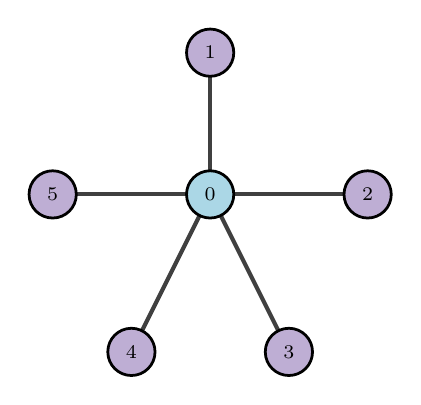
\begin{tikzpicture}
        % Vertices
        \Vertex[x = 0, y = 1.8, label = 1, RGB, color = {190,174,212}]{1}
        \Vertex[x = 0, y = 0, label = 0]{0}
        \Vertex[x = 2, y = 0, label = 2, RGB, color = {190,174,212}]{2}
        \Vertex[x = 1, y = -2, label = 3, RGB, color = {190,174,212}]{3}
        \Vertex[x = -1, y = -2, label = 4, RGB, color = {190,174,212}]{4}
        \Vertex[x = -2, y = 0, label = 5, RGB, color = {190,174,212}]{5}
    
        % Edges
        \Edge(0)(1)
        \Edge(0)(2)
        \Edge(0)(3)
        \Edge(0)(4)
        \Edge(0)(5)
        
        \end{tikzpicture}
        \caption{A Star Network}
        \label{fig:star}
    \end{subfigure}
    % \hfill
    \begin{subfigure}[b]{0.4\textwidth}
        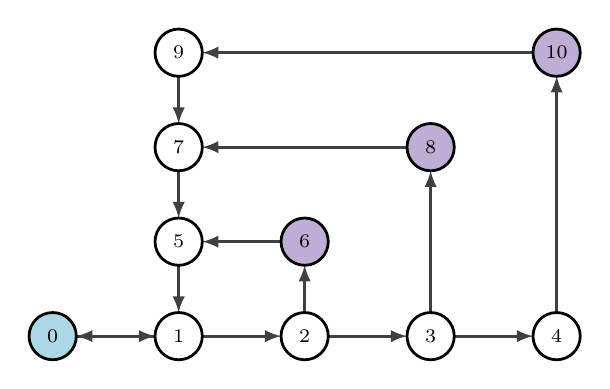
\begin{tikzpicture}
        % Vertices
        \Vertex[x = -4, y = -1.8, label = 0]{0}
        \Vertex[x = -2.4, y = -1.8, label = 1, color = white]{1}
        \Vertex[x = -0.8, y = -1.8, label = 2, color = white]{2}
        \Vertex[x = 0.8, y = -1.8, label = 3, color = white]{3}
        \Vertex[x = 2.4, y = -1.8, label = 4, color = white]{4}
        \Vertex[x = -2.4, y = -0.6, label = 5, color = white]{5}
        \Vertex[x = -0.8, y = -0.6, label = 6, RGB, color = {190,174,212}]{6}
        \Vertex[x = -2.4, y = 0.6, label = 7, color = white]{7}
        \Vertex[x = 0.8, y = 0.6, label = 8, RGB, color = {190,174,212}]{8}
        \Vertex[x = -2.4, y = 1.8, label = 9, color = white]{9}
        \Vertex[x = 2.4, y = 1.8, label = 10, RGB, color = {190,174,212}]{10}
        
        % Edges
        \Edge[lw = 1pt, Direct](0)(1)
        \Edge[lw = 1pt, Direct](1)(0)
        \Edge[lw = 1pt, Direct](1)(2)
        \Edge[lw = 1pt, Direct](2)(3)
        \Edge[lw = 1pt, Direct](3)(4)
        
        \Edge[lw = 1pt, Direct](2)(6)
        \Edge[lw = 1pt, Direct](6)(5)
        \Edge[lw = 1pt, Direct](5)(1)

        \Edge[lw = 1pt, Direct](3)(8)
        \Edge[lw = 1pt, Direct](8)(7)
        \Edge[lw = 1pt, Direct](7)(5)
        
        \Edge[lw = 1pt, Direct](4)(10)
        \Edge[lw = 1pt, Direct](10)(9)
        \Edge[lw = 1pt, Direct](9)(7)
        
        \end{tikzpicture}
        \caption{A One-Way-Dominated Network}
        \label{fig:one-way}
    \end{subfigure}
    \caption{Two types of networks to prove tight upper bounds in Lemma \ref{lemma:1} and Lemma \ref{lemma:2}}
    \label{fig:example_network}
\end{figure}

\propositionk*
\begin{proof}
Suppose $D(m)$ is the set of customers served by vehicle $m$ in the optimal solution and $o$ is the depot. Then, $P(m)$ is the optimal solution to the STSP in the same graph with $D(m) \cup \{o\}$ as the set of required nodes. Based on Lemma \ref{lemma:2}, the upper bound of the number of times $v$ being visited and $(u, v)$ being visited are $|D(m)| + 1$ and $|D(m)|$ respectively. By definition, $k$ is the maximum number of customers vehicle $m$ can potentially serve under any circumstances, meaning that $|D(m)| \leq k$. Thus, the proposition holds.
\end{proof}



\section{Flexible Travel Time for Autonomous Vehicles} \label{Appendix B}
In this section, we further assume an AV is allowed to increase or decrease its speed to some extent when it is cruising along a road segment $(i, j)$. Then, an AV can flexibly adjust the travel time on $(i, j)$ as long as the adjustment is within a threshold, which further enlarges the temporal feasible space of the problem. Define $\underline{\gamma}_{ij}$ ($\overline{\gamma}_{ij}$) as the \textit{minimum (maximum) adjustment factor} for the travel time on road segment $(i, j)$. Then, $[\underline{\gamma}_{ij} \Delta t_{ij}, \;  \overline{\gamma}_{ij} \Delta t_{ij}]$ is the corresponding flexible travel time interval. In this setting, Constraint \ref{c7} in the MILP in Section \ref{sec:milp} is removed and Constraint \ref{c6} is generalized to Constraints \ref{lower} and \ref{upper} for every AV $m \in M^a$. Note that the constraints corresponding to HDVs are kept intact. 
\begin{gather}
    t_{jm} \geq t_{im} + \underline{\gamma}_{ij} \Delta t_{ijm} + T \; (x_{ijm} - 1), \qquad \forall \; (i, j) \in E_e, \; m \in M^a, \label{lower} \\ 
    t_{jm} \leq t_{im} + \overline{\gamma}_{ij} \Delta t_{ijm} + T \; (1 - x_{ijm}), \qquad \forall \; (i, j) \in E_e, \; m \in M^a. \label{upper}
\end{gather}

One may argue that the flexible travel time assumption for the AV fleet is ill-conceived for two reasons: (1) It can impair network efficiency by blocking the traffic in some primary avenues. (2) It can affect the routing cost and change the objective of the problem. For this, we emphasize that it only generalizes the model and provides the possibility to design a better dispatching and routing strategy in the semi-autonomous environment. The adjustment factor of every road segment can be determined separately and designed according to the input network. Also, we admit a linear mapping between the routing cost and the travel time, which makes the problem objective easily adaptable to cases with flexible travel time. 


\subsection{Effects on the Re-Scheduling MILP}
Following the notations used in Section \ref{sec:frp1}, when the flexible travel time assumption is adopted, the time interval of any sub-route $r$ can be independently adjusted by a factor of $\underline{\gamma}_{r}$ for shrinking or $\overline{\gamma}_{r}$ for expanding, where $\underline{\gamma}_r$ and $\overline{\gamma}_r$ are determined in Equations \ref{eq:B1-1} and \ref{eq:B1-2}:
\begin{align}
    \underline{\gamma}_r = \frac{1}{\Delta t_r} \sum_{(i, j) \in r} \underline{\gamma}_{ij} \Delta t_{ij} \label{eq:B1-1}\\
    \overline{\gamma}_r = \frac{1}{\Delta t_r} \sum_{(i, j) \in r} \overline{\gamma}_{ij} \Delta t_{ij} \label{eq:B1-2}
\end{align}

Figure \ref{fig:frp1-1} illustrates how this assumption results in a larger feasible space of the re-scheduling FRP. The original schedules are the same as the ones described in Figure \ref{fig:frp1}, except that the second ordinary sub-route of vehicle $m_1$ is longer. Consequently, the AV-enabled sub-route between the second and the third ordinary sub-routes becomes shorter. In this case, the re-scheduling FRP with fixed travel times is infeasible, as shifting the entire routing schedule of vehicle $m_2$ cannot bypass all overlaps. However, under the flexible travel time assumption, we can further delay the second ordinary sub-route of vehicle $m_2$ by an extra $\delta'$ to eliminate the overlap. This adjustment is equivalent to increasing the travel time of the preceding AV-enabled sub-route by $\delta'$.  
\begin{figure}[!htbp]
    \centering
    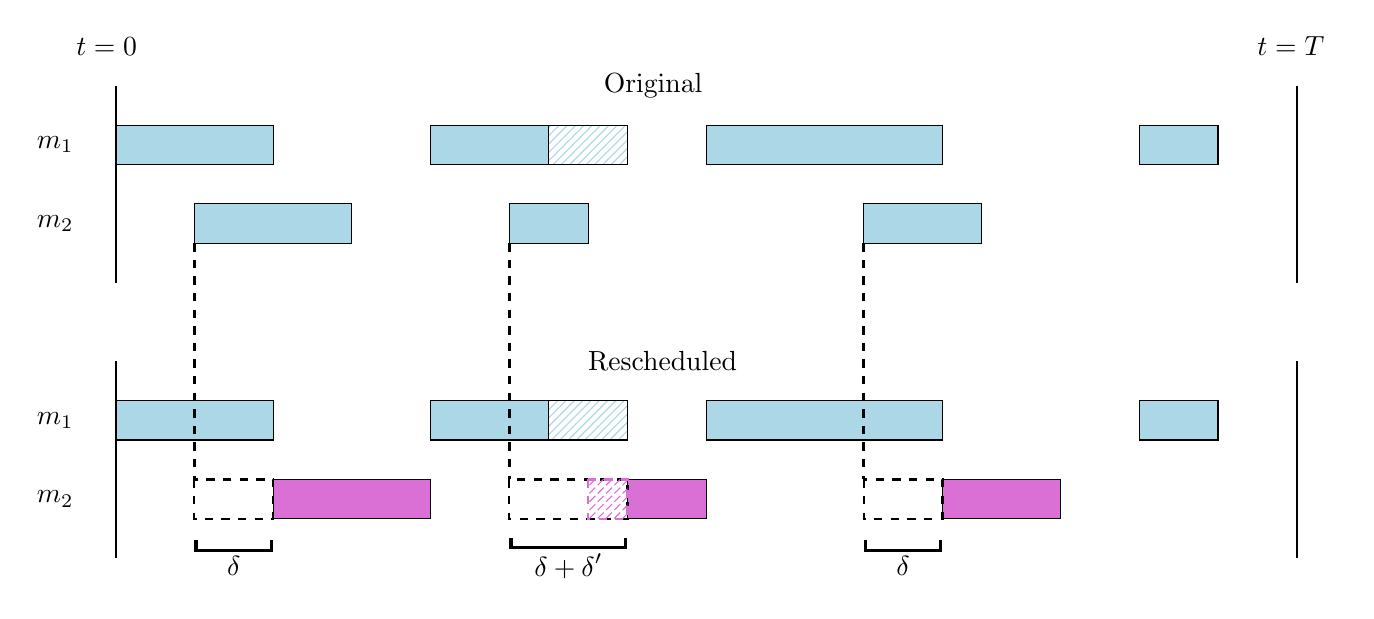
\begin{tikzpicture}

        % Lines
        \draw[thick] (-7, 3) -- (-7, 0.5);
        \draw[thick] (-7, -0.5) -- (-7, -3);
        \draw[thick] (8, 3) -- (8, 0.5);
        \draw[thick] (8, -0.5) -- (8, -3);

        \draw[dashed, very thick] (-6, 1) -- (-6, -2);
        \draw[dashed, very thick] (-2, 1) -- (-2, -2);
        \draw[dashed, very thick] (2.5, 1) -- (2.5, -2);

        % Increase boxes
        \draw[pattern=north east lines, pattern color = vertexfill] (-1.5, 2.5) rectangle (-0.5, 2);
        \draw[pattern=north east lines, pattern color = vertexfill] (-1.5, -1) rectangle (-0.5, -1.5);

        % Delay boxes
        \draw[dashed, thick] (-6, -2) rectangle (-5, -2.5);
        \draw[dashed, thick] (-2, -2) rectangle (-0.5, -2.5);
        \draw[dashed, thick] (2.5, -2) rectangle (3.5, -2.5);
        \draw[dashed, thick, Orchid, pattern=north east lines, pattern color = Orchid] (-1, -2) rectangle (-0.5, -2.5);

        % Text
        \node[text width=1cm] at (-7,3.5) {$t = 0$};
        \node[text width=1cm] at (8,3.5) {$t = T$};
        \node[text width=1cm] at (-7.5, 2.25) {$m_1$};
        \node[text width=1cm] at (-7.5, 1.25) {$m_2$};
        \node[text width=1cm] at (-7.5, -1.25) {$m_1$};
        \node[text width=1cm] at (-7.5, -2.25) {$m_2$};

        \node[text width=2cm] at (0.2, 3) {Original};
        \node[text width=2cm] at (0, -0.5) {Rescheduled};
        
        \node[text width = 2cm] at (-5, -3) {$\underbracket{\hspace{1cm}}_{\displaystyle \delta}$};
        \node[text width = 2cm] at (-1, -3) {$\underbracket{\hspace{1.5cm}}_{\displaystyle \delta + \delta'}$};
        \node[text width = 2cm] at (3.5, -3) {$\underbracket{\hspace{1cm}}_{\displaystyle \delta}$};
        
        \begin{scope}[on background layer]
        % Original
        \filldraw [fill = vertexfill, draw = black] (-7, 2.5) rectangle (-5, 2);
        \filldraw [fill = vertexfill, draw = black] (-3, 2.5) rectangle (-1.5, 2);
        \filldraw [fill = vertexfill, draw = black] (0.5, 2.5) rectangle (3.5, 2);
        \filldraw [fill = vertexfill, draw = black] (6, 2.5) rectangle (7, 2);
        
        \filldraw [fill = vertexfill, draw = black] (-6, 1.5) rectangle (-4, 1);
        \filldraw [fill = vertexfill, draw = black] (-2, 1.5) rectangle (-1, 1);
        \filldraw [fill = vertexfill, draw = black] (2.5, 1.5) rectangle (4, 1);
        
        % Re-scheduled
        \filldraw [fill = vertexfill, draw = black] (-7, -1) rectangle (-5, -1.5);
        \filldraw [fill = vertexfill, draw = black] (-3, -1) rectangle (-1.5, -1.5);
        \filldraw [fill = vertexfill, draw = black] (0.5, -1) rectangle (3.5, -1.5);
        \filldraw [fill = vertexfill, draw = black] (6, -1) rectangle (7, -1.5);
        
        \filldraw [fill = Orchid, draw = black] (-5, -2) rectangle (-3, -2.5);
        \filldraw [fill = Orchid, draw = black] (-0.5, -2) rectangle (0.5, -2.5);
        \filldraw [fill = Orchid, draw = black] (3.5, -2) rectangle (5, -2.5);

        \end{scope}

        % \node[text width=1cm] at (-6.5,2.5) {$t_1$};
        % \node[text width=1cm] at (-3.8,2.5) {$t_2$};
        % \node[text width=1cm] at (-1.5,2.5) {$t_5$};
        % \node[text width=1cm] at (2.2,2.5) {$t_6$};
        % \node[text width=1cm] at (4.5,2.5) {$t_8$};
        % \node[text width=1cm] at (7.2,2.5) {$t_9$};
        
        % \node[text width=1cm] at (-4.9,1.5) {$a_{10}$};
        % \node[text width=1cm] at (0,1.5) {$b_{10}$};
    \end{tikzpicture}
     \caption{The illustration of the re-scheduling FRP with flexible travel time}
    \label{fig:frp1-1}
\end{figure}

To facilitate this more powerful re-scheduling strategy, we can simply relax the hard constraints of fixed travel time accumulation in \ref{frp1:c1} to \ref{frp1:c2} to the soft constraints shown in \ref{frp1:c8} to \ref{frp1:c11}.
\begin{align}
    &t^1_r \leq \overline{t}_m + \sum_{r': \; r' \, \prec \, r} \overline{\gamma}_{r'} \Delta t_{r'}, \qquad r \in R,  \label{frp1:c8} \\
    &t^1_r \geq \overline{t}_m + \sum_{r': \; r' \, \prec \, r} \underline{\gamma}_{r'} \Delta t_{r'}, \qquad r \in R, \label{frp1:c9} \\
    &t_r^2 \leq t_r^1 + \overline{\gamma}_r \Delta t_r, \qquad \forall \; r \in R, \label{frp1:c10} \\
    &t_r^2 \geq t_r^1 + \underline{\gamma}_r \Delta t_r, \qquad \forall \; r \in R.   \label{frp1:c11}
\end{align}

\section{The Re-Routing MILP} \label{Appendix C}
The re-routing MILP takes as input an expanded graph $G_e$, a set of customers $D$, an end time of operation $T$, and a set of \textit{infeasible time intervals} $Q$, where each interval has a start times $a_q$ and an end time $b_q$. During each infeasible time interval, the budget of remote controllers is already exhausted by other AVs. The objective is to find a minimum-cost tour visiting all customers exactly once. 

We adopt most notations from Section \ref{sec:milp} and overwrite the following for simplicity: Define a binary decision variable $x_{ij}$ for every edge $(i, j) \in E_e$ to indicate whether the edge is selected in the route. Define a binary decision variable $y_i$ for every customer $i \in D_e$ to indicate whether a duplicate of the customer in the expanded graph is served. Define a continuous variable $t_i \in [0, T]$ for every node $i \in V_e$ to represent the timestamp of the AV visiting the node. Define a binary decision variable $\alpha_{qij}$ for every $q \in Q$ and every edge $(i, j) \in E_e$, with $\alpha_{qij} = 1$ indicating the timestamp of the vehicle exiting edge $(i, j)$ is later than the start time of interval $q$. Define a binary decision variable $\beta_{qij}$ for every $q \in Q$ and every edge $(i, j) \in E_e$, with $\beta_{qij} = 1$ indicating the timestamp of the vehicle entering edge $(i, j)$ is earlier than the end time of interval $q$. Then, the re-routing MILP can be formulated as follows.  
\begin{mini}|s|[2]<b>
    {\bm{x}, \bm{y}, \bm{t}, \bm{\alpha}, \bm{\beta}} 
    {\sum_{(i, j) \in E^a_e} c_{ij}^1 x_{ij} + \sum_{(i, j) \in E^o_e} c_{ij}^2 x_{ij}}{}{}
    \addConstraint{\sum_{j \in \delta^-(i)} x_{ij}}{= \sum_{j \in \delta^+(i)} x_{ji}, \quad}{\forall \; i \in V_e - \{o, s\}}
    \addConstraint{\sum_{j \in \delta^-(o)} x_{oj} = \sum_{j \in \delta^+(s)} x_{js} \leq 1,}{}
    \addConstraint{\sum_{i \in D^V(j)} y_{i}}{= 1, \quad}{\forall \; j \in D}
    \addConstraint{\sum_{j \in \delta^+(i)} x_{ji}}{\geq y_{i}, \quad}{\forall \; i \in D_e}
    \addConstraint{x_{ij}}{\leq y_{i}, \quad}{\forall \; (i, j) \in A}
    \addConstraint{t_{j}}{\geq t_{i} + \Delta t_{ij} + T (x_{ij} - 1), \quad}{\forall \; (i, j) \in E_e}
    \addConstraint{t_{s}}{= t_{o} + \sum_{(i,j) \in E_e} \Delta t_{ij} x_{ij} \leq T}
    \addConstraint{t_{j}}{\leq a_q + T \alpha_{qij}, \quad}{\forall \; q \in Q, \forall \; (i, j) \in E^o_e}
    \addConstraint{t_{j}}{\geq a_q + T (\alpha_{qij} - 1), \quad}{\forall \; q \in Q, \forall \; (i, j) \in E^o_e}
    \addConstraint{b_q}{\leq t_{i} + T \beta_{qij}, \quad}{\forall \; q \in Q, \forall \; (i, j) \in E^o_e}
    \addConstraint{b_q}{\geq t_{i} + T (\beta_{qij} - 1), \quad}{\forall \; q \in Q, \forall \; (i, j) \in E^o_e}
    \addConstraint{\alpha_{qij} + \beta_{qij} + x_{ij}}{\leq 2, \quad}{\forall \; q \in Q, \forall \; (i, j) \in E^o_e}
\end{mini}

\section{Experimental Results} \label{Appendix D}
The rounded routing costs for the VRP-SA instances, which correspond to Figure \ref{fig:main_result}, are listed in Table \ref{tab:main_result} below.
\renewcommand{\arraystretch}{1.3}
\begin{longtable}{c|c|cc}
    \caption{Routing cost for the VRP-SA instances} \label{tab:main_result} \\ \hline
    \multirow{2}{*}{\textbf{Instances}} & \multirow{2}{*}{\textbf{Cost by HDVs}} & \multicolumn{2}{|c}{\textbf{Cost by HDVs + AVs}}  \\ \cline{3-4}
    & & \textbf{w.o. re-routing priority} & \textbf{w. re-routing priority} \\ \hline
    \endfirsthead

    \hline
    \multirow{2}{*}{\textbf{Instances}} & \multirow{2}{*}{\textbf{Cost by HDVs}} & \multicolumn{2}{|c}{\textbf{Cost by HDVs + AVs}}  \\ \cline{3-4}
    & & w.o. re-routing priority & w. re-routing priority \\ \hline
    \endhead

    \hline
    \endfoot

    \hline
    \endlastfoot

    P-n16-k8 & 600 & 387 & 386 \\
    P-n19-k2 & 280 & 251 & 247 \\
    P-n20-k2 & 282 & 249 & 249 \\
    P-n21-k2 & 282 & 258 & 258 \\
    P-n22-k2 & 288 & 269 & 243 \\
    P-n22-k8 & 750 & 508 & 472 \\
    P-n23-k8 & 694 & 474 & 475\\
    P-n40-k5 & 590 & 501 & 455\\
    P-n45-k5 & 650 & 563 & 532 \\
    P-n50-k7 & 700 & 645 & 579 \\
    P-n50-k8 & 798 & 627 & 624 \\
    P-n50-k10 & 880 & 682 & 680\\
    P-n51-k10 & 958 & 779 & 755 \\
    P-n55-k7 & 710 & 615 & 601\\
    P-n55-k10 & 870 & 685 & 689 \\
    P-n55-k15 & 1204 & 895 & 880\\
    P-n60-k10 & 926 & 876 & 856 \\
    P-n60-k15 & 1230 & 971 & 963 \\
    P-n65-k10 & 992 & 928 & 913 \\
    P-n70-k10 & 1034 & 988 & 926 \\
    P-n76-k4 & 742 & 759 & 722\\
    P-n76-k5 & 780 & 772 & 766 \\
    P-n101-k4 & 876 & 857 & 878 \\ 
\end{longtable}
\end{document}